\documentclass[a4paper,10pt]{report}

\usepackage[utf8]{inputenc}
\usepackage{xspace}
\usepackage{graphicx,graphics} 
\usepackage{color}
\usepackage{amsmath}
\usepackage{amsfonts}
\usepackage{amssymb}
\usepackage{amsthm}
\usepackage{algorithm}
\usepackage{algorithmic}
\usepackage{longtable}
\usepackage{complexity}
\usepackage{tkz-graph}
\usepackage{float}
\usepackage{setspace}
\renewcommand{\algorithmicrequire}{\textbf{Input:}}
\renewcommand{\algorithmicensure}{\textbf{Output:}}
  
\graphicspath{{figures/}}
\newcommand\rmatching{${\cal R}$-matching\xspace}
\newcommand\mdelay{$\cal M$-delay\xspace}
\newcommand\matchedgraph{{\bf matched graph}}

\newcommand{\reporttitle}{Latency management for Deterministic Networking}     % Titre
\newcommand{\reportauthor}{Maël \textsc{Guiraud }} % Auteur
\newcommand{\reportsubject}{Graduation Memoir} 
\newcommand{\HRule}{\rule{\linewidth}{0.5mm}}
\setlength{\parskip}{1ex} % Espace entre les paragraphes

\newcommand{\todo}[1]{}
\renewcommand{\todo}[1]{{\color{red} TODO: {#1}}}
\begin{document}
\begin{titlepage}

\begin{center}



\begin{minipage}[t]{0.48\textwidth}
  \begin{flushleft} \large
       
\includegraphics [width=50mm]{logo.png} \\[0.5cm]
  \end{flushleft}
\end{minipage}
\begin{minipage}[t]{0.48\textwidth}
  \begin{flushright} \large
    
\includegraphics [width=50mm]{logon.png} \\[0.5cm]
  \end{flushright}
\end{minipage}
 \\[3cm]

\textsc{\Large \reportsubject}\\[0.5cm]
\HRule \\[0.4cm]
{\huge \bfseries \reporttitle}\\[0.4cm]
\HRule \\[1.5cm]

\begin{minipage}[t]{1.0\textwidth}
  \begin{center} \large
    \emph{Master 2:} 
   Algorithmique et Modélisation à l'Interface des Sciences(AMIS) \\

  \end{center}
  \end{minipage}
  \\[3cm]
 
\begin{minipage}[t]{0.3\textwidth}
  \begin{flushleft} \large
    \emph{Student:}\\
    \reportauthor 
  \end{flushleft}
\end{minipage}
\begin{minipage}[t]{0.6\textwidth}
  \begin{flushright} \large
    \emph{Supervisors:} \\
    Dominique \textsc{Barth} \\
    Olivier \textsc{Marcé} \\
    Yann \textsc{Strozecki} \\
    Christian \textsc{Cadéré} \\

  \end{flushright}
\end{minipage}

\vfill

{\large September 2016}

\end{center}

\end{titlepage}

\newpage
\null
\newpage

\section*{Acknowledgements}
This internship takes place in a collaboration between the laboratories DAVID and Nokia Bell Labs France.
The project would not have been possible without the trust of my professor Dominique Barth and supervisor Olivier Marcé, thit is why i would like to express my gratitude to them for the time they spent in this project with me.\\

I would also like to thank Yann Strozecki and Christian Cadéré for following and supervising closely my work, and providing me many advice that allowed me to work in optimal conditions.

I also express my appreciations to the teams of DAVID and Nokia Bell Labs for their warm welcome and advice.
\tableofcontents

\begin{chapter}{Overview of the internship}
\begin{section}{Company}
Nokia is a global leader in the technologies that connect people and things. Powered by the innovation of Nokia Bell Labs and Nokia Technologies, the company is at the forefront of creating and licensing the technologies that are increasingly at the heart of our connected lives. With state-of-the-art software, hardware and services for any type of network, Nokia is uniquely positioned to help communication service providers, governments, and large enterprises deliver on the promise of 5G, the Cloud and the Internet of Things. Nokia is combining its own proud R\&D heritage with the unrivalled history of Nokia Bell Labs. Nokia Bell Labs is the research and innovation arm of Nokia which has been awarded 8 Nobel prizes over its lifetime, together creating around 31 000 patent families. Nokia Bell Labs mission is to define the future of communications and networking and deliver disruptive innovations that redefine human existence and business realities.
Nokia Bell Labs France, the French Nokia Bell Labs center and the second in size, is located in Nokia Paris-Saclay ``Innovation City``, in Nozay close to Paris. The Nokia Paris-Saclay ''Innovation City`` is a large R\&D location open to its ecosystems and partners, and is located in the vicinity of Paris-Saclay campus. Nokia Bell Labs France is covering research on III-V photonics devices, optical transmission and signal processing, IP and optical networking, end to end mobile network solutions, software defined wireless networks, networks algorithms and control, cyber security, analytics and mathematics of complex dynamic networks. Nokia Bell Labs France hosts also a team in charge of maturation of research results, and ''Le Garage``, a dedicated space that fosters the ''startup`` spirit. As part of the open innovation strategy of Nokia Bell Labs, Nokia Bell Labs France is also highly active in collaborative programs, research partnerships, and joint research laboratories.
\end{section}
\begin{section}{Context}
The current mobile network architecture consists in distributed radio access networks.
The evolutions proposed in next generations aim to build centralised radio network architectures (C-RAN) to reduce consumption costs 
and power at the base stations. These C-RAN architectures include simplified base stations at each antenna (Remote Radio Heads: RRH) 
and central processing units (baseband unit: BBU) located in the cloud. Thus, this type of architecture confronts the problem of controlling 
the latency in the transfer process.  Low latency is considered critical for the 5G, in particular for the deployment of the C-RAN approach 
(allowing time constraints like HARQ to be fulfilled over non dedicated networks), or to reach E2E expected latency from 1 to 10ms 
(depending on targeted services). One specificity in the C-RAN context is not only the latency constraint, but also the periodicity of 
the data transfer between RRH and BBU.  New scheduling and routing paradigms and new technologies have to be considered to  guarantee 
delay constrained periodic data transfers. Dynamical optical bypass and dynamical management of the emission should be considered to
guarantee latency constraints. This is why this study is a contribution to the ANR project N-Green.

N-GREEN proposes a new type of switching/routing node and a specific network architecture exploiting WDM packets thanks to a new generation of optical add/drop multiplexers (WSADM: WDM slotted add/drop multiplexer). These packets having a fixed duration close to 1 µs are transported in a transparent way, to better exploit the switching matrix of the node; their headers will be transported over one dedicated wavelength at a lower bit rate, to reduce the physical constraints of the electronic processing and scheduler.

 Thus, this subject targets new scheduling and routing paradigms to solve this periodic and delay constrained data transfer.
 Indeed, one of the most promising approaches relies on the concept of Deterministic Networking (DN) such that one get rid of
 statistical multiplexing. The traditional queue managements are replaced by time based forwarding. Solutions for Deterministic 
 Networking are under standardization in IEEE 802.1 TSN group, as well at IETF DetNet working group.  To make DN working over a
 network composed of several nodes, it is required to manage the time at which the packets of deterministic paths are crossing each nodes. 

Considering a graph, modelling the network topology, and a set of routes from source nodes (modelling connections to the BBU) and destination 
nodes (modelling the RRH) in this graph, the purpose is to select, for each destination node a route from one source node to it and a periodic 
routing scheme allowing to periodically sent a packet to each base station without congestion conflicts between all such packets and to insure a minimum latency. In a slotted time model, the aim is here to minimize the duration of the period, with a constraint of the maximum length of routes to be
selected. Even if the selected set of routes is given this optimisation problem has been shown to be  \NP-hard. From an algorithmic point of view,
the purpose of this project is first, to study the complexity and the approximability of this problem when the length of the routes is small
(which corresponds to realistic cases), and secondly, to propose and implement some heuristics to solve this problem on realistic topologies.


The major difficulty of this problem is the periodicity of the process. Indeed, a deterministic sending for the messages
between each pair BBU/RRH must consider the other messages sent by the others BBU/RRH in the same period, but also in the previous
and following periods. The issue is due to the different length of the paths. This problem may look like wormhole problem \cite{cole1996benefit}, very popular few years ago, but here, we want to minimize the time lost in buffers and not just avoid the deadlock, and the wormhole does not treat about the periodicity.
\end{section}

\end{chapter}

\begin{chapter}{Periodic assignment problem}
 In this chapter we will introduce the modelling of the network by graphs. This report uses classical notions of graph theory basic definitions that you can find in the book ``Graph Theory'' by Reinhard Diestel \cite{diestel2005graph}.
 \begin{section}{Model}
 \begin{subsection}{Definitions}
  A Fronthaul network can be considered as a directed graph $G=(V,A)$ with two non intersecting subsets of vertices: 
  a subset $L$ of nodes which are called {\bf leaves} and a subset $S$ of nodes which are called {\bf sources}.  
The indegree of nodes in $S$, and the outdegree of nodes in $L$ are equal to 0. 
We denote by ${\cal L}$ the cardinal of $L$ and by ${\cal S}$ the cardinal of $S$. The digraph $G$ models the network,
$S$ is the set of BBU and $L$ is the set of RRH. The others nodes of the graph are the switches.
Each arc  $(u,v)$ in $A$ has an integer weight $Dl(u,v) \geq 1$ representing the time taken by the signal to go from $u$ to $v$
 using this arc.

We consider $G^r=(V,A^r)$ wherein the set of vertices is the same as in $G$, and $A^r$ represents the edges of $A$ directed in the other way. 
\newline
\begin{center}
\fbox{\parbox{11cm}{
\begin{figure}[H]
\begin{center}
\begin{tabular}{cc}
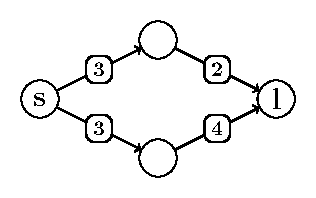
\includegraphics[scale=0.8]{Fig2.pdf} & 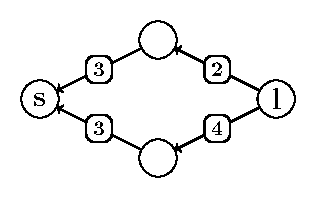
\includegraphics[scale=0.8]{Fig3.pdf}\\
 $G=(V,A)$ & $G^r=(V,A^r)$\\
\end{tabular}
\end{center}
\end{figure}

}}\end{center}

A {\bf route} $r$ is a sequence of arcs $a_0, \ldots , a_{n-1}$, with $a_i=(u_i,u_{i+1}) \in A$ such that $u_0 \in L$ and $u_n \in S$.
The {\bf latency} of a vertex $u_i$ in $r$, with $i \geq 1$, is defined by $$\lambda(u_i,r)= \sum\limits_{0 \leq k <i} Dl(a_k)$$ We also define $\lambda(u_0,r)=0$.
The latency of the route $r$ is defined by $\lambda (r)= \lambda (u_n,r)$. In graph theory, a route is a simple path in the graph, and its latency is its weight. 


A {\bf routing function}  ${\cal R}$ is an application associating a route  ${\cal R}(s,l)$ to each couple $(s,l) \in S \times L$ in $G$.
Moreover ${\cal R}$ satisfies the {\bf coherent routing} property: the intersection of two routes must be a path.

For simplicity, we assume that we have as many source nodes as we have leaves (${\cal S} = {\cal L})$.
A {\bf ${\cal R}$-matching} is a bijection $\rho:S\rightarrow L$ which associates to each $s_i \in \{s_0,...,s_{{\cal S}-1}\}$ 
a $l_i \in \{l_0,...,l_{{\cal L}-1}\}$.
A \rmatching defines a set $\{r_0, \ldots ,r_{{\cal L}-1}\}$ of ${\cal L}$ routes in ${\cal R}$ such that $\forall i\,, r_i = {\cal R}(s_i,l_i)$.

The quintuplet $N=(G,S,L,{\cal R},\rho)$ defines a \matchedgraph. We call $N^r$ the quintuplet $(G^r,S,L,{\cal R},\rho^r)$, 
where $\rho^r$ is the \rmatching obtained using the same routes, with inverted arcs.

\end{subsection}
\begin{subsection}{Slotted time Model}
\label{slottedtime}
In our model, the time is discrete. The unit of time is one slot. Two values are expressed in time slots: 
\begin{enumerate}
 \item The emission time of a message by a node, the {\bf message length}, We denote by {\bf T} this time.
 \item The time taken by a message to cross a link, the {\bf delay} of an arc.
\end{enumerate}

Let $P>0$ be an integer called {\bf period}. 
A $P$-periodic affectation of N(a matched graph) consists in a set  ${\cal M}=(m_0, \ldots ,m_{{\cal L}-1})$
of ${\cal L}$ integers that we call {\bf offset}. 
Each period is divided in $P$ slots and the number $m_i$ represents the first slot number used by the route $r_i$ at its source.
We define the first time slot at which a message arrive at any vertex $v$ of the route by $$t(v,r_i) = m_i+\lambda(u,r_i) \mod P.$$

Let us call $[t(v,r_i)]_{T,P}$ the values of the time slots used by a route $r_i$ in a vertex $v$. 
Those values are forming a continuous set of values starting at $t(v,r_i) \mod P$ and ending at $t(v,r_i) + T \mod P$.
For a given instance, $P$ and T does not change at any moment, indeed, the size of the messages is the same for any route, and the period is also the same for any vertex.
So, since $P$ and T are fixed, we simplify the notation by $[t(v,r_i)]$.

A $P$-periodic affectation must have no {\bf collision} between two routes in $\rho$, that is $\forall r_i, r_j \in \rho, i \ne j$,
we have $$[t(u,r_i)] \cap [t(u,r_j)] = \emptyset .$$

\fbox{\parbox{12cm}{
Notice that the notion of $P$-periodic affectation \textbf{is not monotone} with regard to $P$. 
Indeed, we can build a {\bf ${\cal R}$-matching} of a graph, with ${\cal L}$ routes $r_1, \dots, r_l$ which all intersect two by two and
such that if $r_i$ and $r_j$ have $v$ as first common vertex we have $\lambda(v,r_i) - \lambda(v,r_j)=1$.
Therefore there is a $2$-periodic affectation by setting all $m_i$ to $0$.

A {\bf conflict graph} represents the collision between the routes in the matched. The vertices of a conflict graph $G = (V,E)$ are the routes, and there is an edge between two vertices if and only if there is a common arc between the two routes in the matched graph.
 
 Given $u$ and $v$ two vertices of the conflict graph, corresponding to two routes colliding in the matched graph. The weight $w(u,v)$ of an edge is the difference between the distance of the two routes between their respective source node and the collision point.
 
 A labelling $F$ of such a graph is an affectation of an integer to each vertex, such that for each vertex $u$, $f(u) \neq f(v)+w(u,v)\mod P$, where $v$ are the neighbours of $u$ in the conflict graph and $P$ our period.
 
\begin{tabular}{cc}
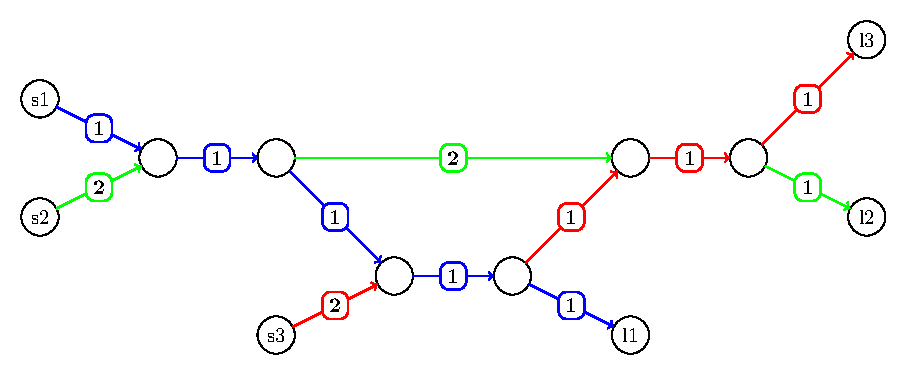
\includegraphics[scale=0.5]{Fig5.pdf} & 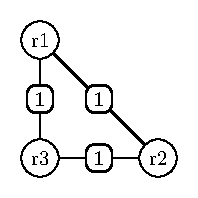
\includegraphics[scale=1]{Fig7.pdf}\\
 $\lambda(v,r_i) - \lambda(v,r_j)=1$ & Conflict graph\\
\end{tabular}\newline

On the other hand if we set all $\lambda(v,r_i) - \lambda(v,r_j)=P$, there is no $P$-periodic affectation if $P<l$.

\begin{tabular}{cc}
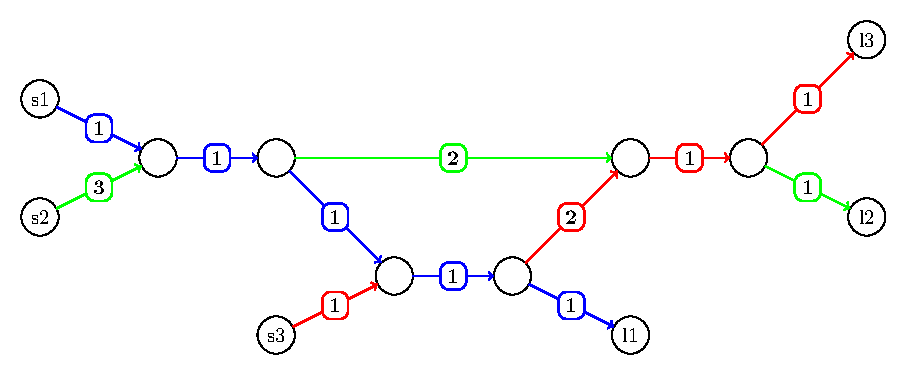
\includegraphics[scale=0.5]{Fig6.pdf} & 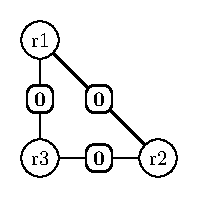
\includegraphics[scale=1]{Fig8.pdf}\\
 $\lambda(v,r_i) - \lambda(v,r_j)=2$ & Conflict graph\\
\end{tabular}\newline
\begin{center}
 Here for P=2, there is no $P$-periodic affectation.
\end{center}

Therefore if we choose and odd value for $P$ and $l=P+1$, there is no $P$-periodic affectation but modulo $2$ all $\lambda(v,r_i) - \lambda(v,r_j)$
are equal to one thus we have a $2$-periodic affectation. 
}}
\end{subsection}
\begin{subsection}{Topology}

This project focuses on the analysis of a fronthaul network. In those kinds of networks, we can differentiate three kinds of
topologies. Each one of them correspond to a real configuration, depending of the distance between the BBU and the RRH.
\begin{enumerate}
 \item Topology 1: A basic network topology, composed of some base stations, represented by source nodes $S$, all connected to the same switch,
which will be a vertex, connected itself to another vertex, corresponding to a switch, connected to some leave nodes $L$ representing the RRH.
\item Topology 2: A network containing an optical ring, such that some sources nodes be connected to it anywhere, not intersecting themselves before the ring,
and some set of leave nodes are also connected at any point of the ring.
\item Topology 3: The general case: A DAG, on which we may restrict parameters as the degree or the number of vertices to represent graphs corresponding to realistic networks.
\end{enumerate}
\fbox{\parbox{12cm}{
\begin{figure}[H]

\begin{center}
 
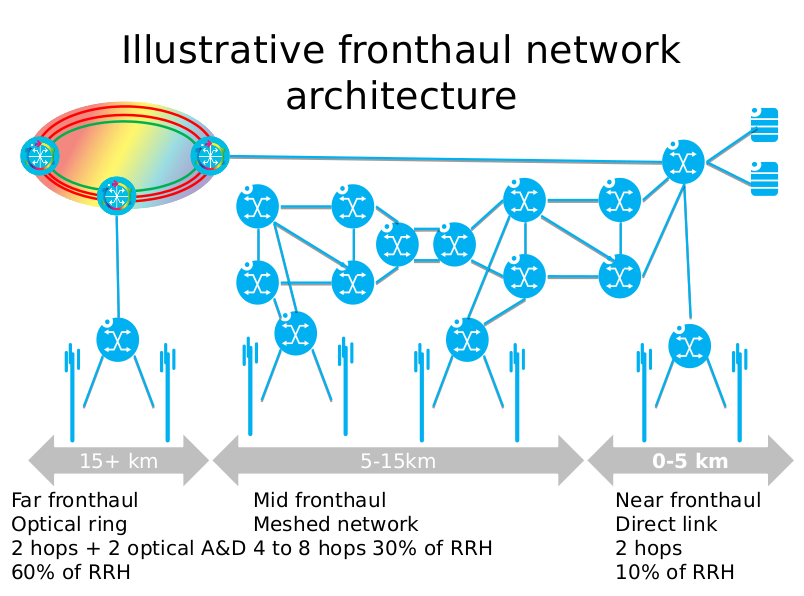
\includegraphics[scale=0.4]{fronthaul0.png}\\

\end{center}
\caption{From left to right: Topologies 2, 3 and 1 representing respectively the far, mid and near fronthaul.}
\end{figure}
}}\\

This report focus on studying the first topology, which is already rich enough to yield interesting questions.

\end{subsection}

\end{section}
\begin{section}{Problem}
   
The application we address here by studying the problems defined above is the following. Consider a fronthaul network in which source nodes in $S$ represent BBU.
Each of the source nodes do a computation for its associated RRH represented by a leaf node in $L$. Consider a ${\cal R}$-matching $\rho$ of $S$ in $L$. Consider a leaf $l$, its dedicated source node $s$
and $R(l,s)$ the route from $l$ to $s$ in $R$. We consider a $P$-periodic affectation of N, and also another $P$-periodic affectation of $N^{r}$.
The periodic process is, for each route, the following one:
\begin{enumerate}
 \item During each period of duration $P$, $l$ sends a message to its source $s=\rho(l)$, using its routes according to the $P$-periodic affectation of N. 
 \item When a source $s=\rho(l)$ receive a message from $l$, it makes a computation. This computation time is the same for all sources.
 \item After this computation time, $s$ sends a message to $l=\rho(l)$ according to the $P$-periodic affectation of $N^{r}$.
\end{enumerate}

\fbox{\parbox{11cm}{
\begin{center}
\scalebox{0.6}{
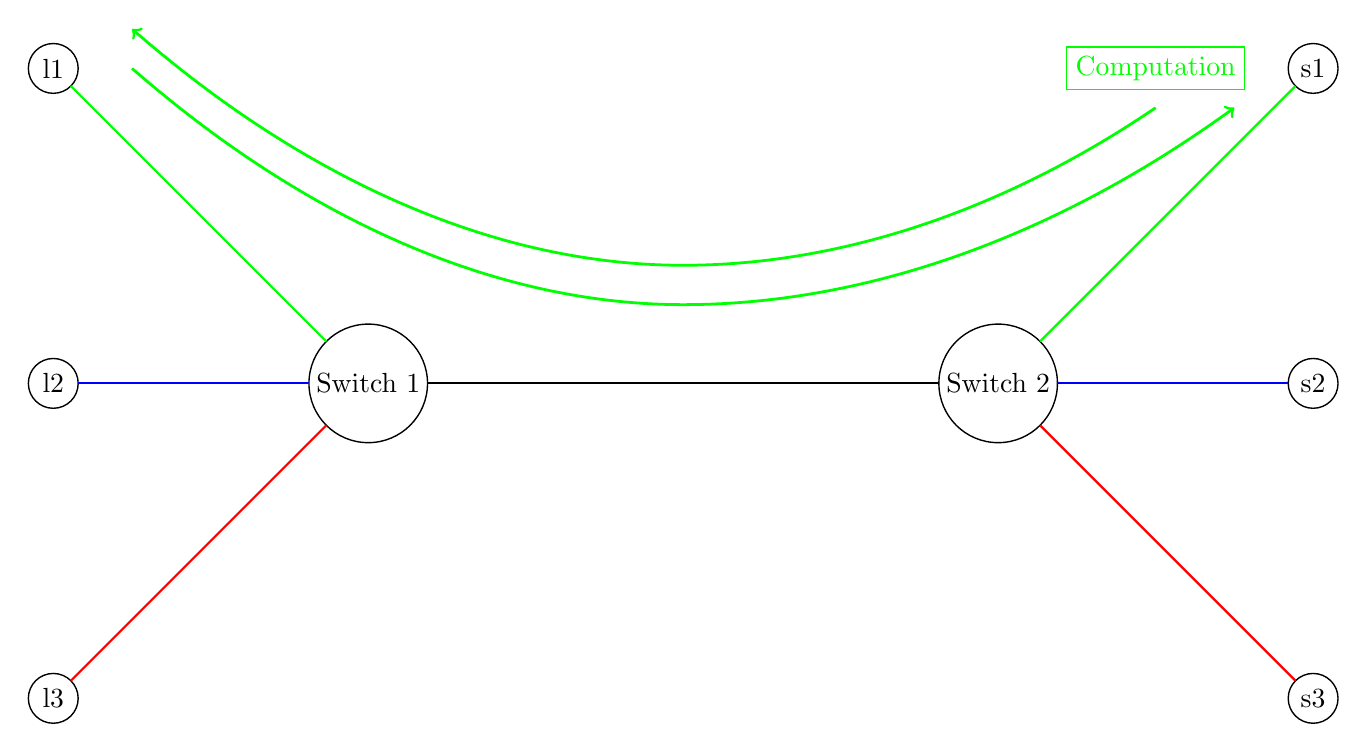
\begin{tikzpicture}
  \SetGraphUnit{5}
  \Vertex[x=0,y=0]{l3}
  \Vertex[x=0,y=4]{l2}
  \Vertex[x=0,y=8]{l1}
  
  \Vertex[x=16,y=0]{s3}
  \Vertex[x=16,y=4]{s2}
  \Vertex[x=16,y=8]{s1}
  
  \Vertex[x=4,y=4]{Switch 1}
  \Vertex[x=12,y=4]{Switch 2}  
  \tikzset{
  EdgeStyle/.append style = {green} }
  \Edge(s1)(Switch 2)
  \Edge(Switch 1)(l1)
  
  \tikzset{
  EdgeStyle/.append style = {blue} }
  \Edge(s2)(Switch 2)
  \Edge(Switch 1)(l2)
  
  \tikzset{
  EdgeStyle/.append style = {red} }
  \Edge(s3)(Switch 2)
  \Edge(Switch 1)(l3)
  
  \tikzset{
  EdgeStyle/.append style = {black} }
  \Edge(Switch 1)(Switch 2)
  
  \draw[->,line width=1pt,green] (1,8) parabola bend (8,5) (15,7.5);
  \node[draw,green] at (14,8) {Computation};
  \draw[<-,line width=1pt,green] (1,8.5) parabola bend (8,5.5) (14,7.5);


\end{tikzpicture}
}
\end{center}}}\\

On source nodes, between the end of the computation time and the emission time of the message (given by the $P$-periodic affectation), there is a {\bf waiting time}. 
We define by $\omega: r \rightarrow \mathbb{N}$ the waiting time of a route $r$ in the ${\cal R}$-matching considered, i.e. the time during which the
message is ''sleeping``, waiting to be sent through the network.


We have to find two $P$-periodic affectations, one for the messages going from the RRH to the BBU, and another one for the answers going from BBU to the RRH. Those two $P$-periodic affectations have the same period $P$. 
If the messages have to be buffered, we can only do it in sources nodes.
We define by $\theta$ the computation time required at the source node before sending an answer to its leaf node.

A {\bf TwoWayTrip} is, for a route, the full travel leaf-leaf, including the waiting time and the computation time.

Let us call $T (r)$ the time of a TwoWayTrip on a route $r$: $$ T (r) = 2\lambda (r) + \omega (r) + \theta$$

Since $\theta$ is the same on every route, we can simplify the model by removing $\theta$. Whether we want to consider it, we only have to lengthen all 
links before source nodes by $\frac{\theta}{2}$. 


In our network application, since $P$ and the ${\cal R}-matching$ are given, we do not need to minimize $P$.
Therefore we want to optimise the time taken by the messages to do the TwoWayTrip in order to ensure a good level of quality of service.

A {\bf TwoWayTrip affectation} of $N$ is a set of pairs $ ((m_0,x_0),...,(m_{{\cal L}-1},x_{{\cal L}-1}))$ in which ${\cal M} = (m_0,...,m_{{\cal L}-1})$ 
is a $P$-periodic affectation of $N$,${\cal X} = (x_0,...,x_{{\cal L}-1})$ is a $P$-periodic affectation of $N^r$, and we define the waiting time of the route $r_i$ by:
$$ \omega_i = x_i - (m_i + \lambda(r_i)) \mod P .$$ 

Since ${\cal M}$ and ${\cal X}$ are some $P$-periodic affectation, they must have no collisions as we have already defined.

% In this topology, once the first central switch passed, there is no more possible collisions between two routes, so, 
% there is an unique vertex on each matched graph N or N$^r$ on which a collision is possible.
% We can simplify the notation of  $[t(u,r_i)]$ by $[t(i)]$, where $[t(i)]$ is the interval taken by the route $r_i$
% in the conflict point of the matched graph corresponding to the $P$-periodic affectation.


In the network problem, it is not allowed to have a route such that $T(r) > D$. This maximal value $D$ is called the {\bf deadline}.
Thus, the problem we want to solve is the following:\\

\noindent {\bf Periodic Assignment for Low Latency (PALL)} 

\noindent {\bf Input:} Matched graph $N$, integer $P$, $ T_{max}$.

\noindent {\bf Question:} does there exist a TwoWayTrip affectation of $N$, such that $\forall r \in \rho$, $T(r) \le T_{max}$.

Once this decision problem established, we can consider two optimisation problems, derived from the previous problem in which
we try to minimize different functions of $T(r)$.\\

\noindent {\bf Optimization goal 1:} minimizing max($T(r)$).

Minimizing the longest TwoWayTrip time of all routes allows us to win some time, and consequently some distance between the BBU and the RRH.\\

\noindent {\bf Optimization goal 2:} minimizing $\sum_{r \in \rho}  T(r)$ (equivalent to minimizing $\sum_{r \in \rho}  \omega(r)$.

By minimizing the sum of all the routes, we allow a better global Quality of Service through the network.\\
\begin{subsection}{Restrictions of topology 1}
\label{topologiescases}
\fbox{\parbox{12cm}{
 \begin{figure}[H]
\begin{center}

 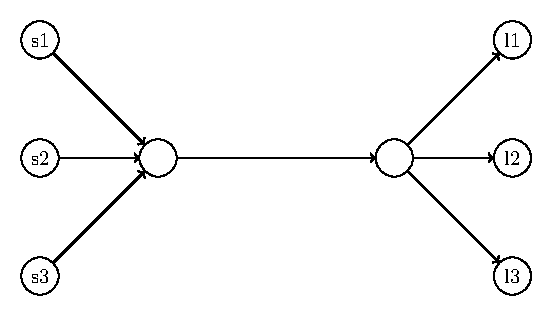
\includegraphics[scale=1]{Fig4.pdf}\\
  \caption{Example of topology 1.}
 
\end{center}
\end{figure}
}}\\


In the considered topology, there are 3 cases:
\begin{enumerate}
 \item When the weights of the links from source nodes are all equal. This is the closest case to the reality, and also the easier to solve.
 \item When the weights of the leave nodes links are all equal.
 \item When all the links have different weights.
\end{enumerate}

The middle switches, denoted by {\bf LS} and {\bf SS} are called respectively {\bf leave switch} and {\bf sources switch}.

The middle link can be represented without weight, because it is common to all the routes and has no influence over the values of T(r), so it can be simplified in computation. 

\end{subsection}
\end{section}
\begin{section}{Related Work}

The following articles helped us to approach our problem, but they all have some common limits next to our problem:
\begin{enumerate}
 \item Articles about coloration considers the messages as one slot it their slotted time. In our situation, it is hard to represent the messages as one slot because our messages are modelled by many slots, and the messages can take many different beginning offsets.
 \item Some articles give us an idea how to find a $P$-periodic affectation, but can not be used to model a TwoWayTrip. 
 \item Except the Circular-coloring, none of these problems deal with the periodicity while it is one of the most important point of our problem.
 
\end{enumerate}

\begin{subsection}{Path Coloring and Call Scheduling}
Let us describe an article of Thomas Erlebach and Klaus Jansen about the Path coloring and Call Scheduling \cite{erlebach2001complexity}.

\paragraph{Path Coloring}
The authors try to solve the scheduling of messages over optical networks. A connection between two nodes must be established, by reserving a wavelength on all links of the
path between the two nodes. The number of wavelengths is limited, so it is necessary to find a way to use the minimum number of wavelengths for a set 
of connections.

The model used is a graph $G=(V,E)$ in which the vertices represent the switches and the links are modelled by the edges. The goal is to give to each
couple of vertex (u,v), a path and a color representing the connection, such that any other couple using a common edge in its path has not the same
color than (u,v). The problem called path coloring is to minimize the number of color used.

Applied to our problem, path coloring gives a different color to each couple BBU/RRH, because they all share the same common link.
Due to our central common links, each color of the path coloring
would correspond to a message in our problem. Considering our slotted time model in which a message uses more than one slot,
it is hard to fit our model in path scheduling model.

Furthermore this approach does not treat the periodicity. 

\paragraph{Call Scheduling}
In bandwidth reservation networks, the links have different bandwidths and each message 
needs a different bandwidth to be transmitted. The call scheduling problem is to set the paths and the starting times of the connection requests.
The goal is to minimize the latest completion time i.e. the moment in which all the messages are transmitted.

To solve this problem, the authors are using a graph $G=(V,E)$, in which the edges have a capacity representing the bandwidth.
A call is represented by a couple (u,v) of vertices, a bandwidth requirement and a duration. The goal is to give a starting time to each call
such that any call has enough bandwidth on its links when it is active.

In our problem all the bandwidth requirements, call durations and edge capacities are the same.
On the other hand, solving call scheduling does not solve our TwoWayTrip problem, since it only deals with one $P$-periodic affectation of the TwoWayTrip and does not take into account the periodicity.

Furthermore, this article does not give a polynomial algorithm to solve path coloring or call scheduling. 

Path Coloring is shown as \NP-hard for bi-directed trees. Call Scheduling is \NP-hard for almost all network topology. Even with a good reduction of our problem in one of those, we would have not find a polynomial algorithm.


\end{subsection}

\begin{subsection}{A fast algorithm for single processor scheduling}
The article ''A fast algorithm for single processor scheduling`` \cite{simons1978fast}, by Barbara Simons presents an efficient algorithm for task 
scheduling on a single processor. All the tasks have the same execution time. The complexity of this algorithm is $O(n^2\log(n))$, n is the number of tasks.

This algorithm considers a set of tasks which have a release time and a deadline. The goal is to schedule the tasks on a single processor such
that each task does not start before its release time and stop before its deadline.
A scheduling is a set of starting times for the tasks which satisfies the previous conditions.
The algorithm finds a solution, if it exists, which minimizes the time at which the last task is completed.

The algorithm is divided in three parts.
The main algorithm which schedules the task in a greedy way, by selecting the task according to two criteria:
\begin{enumerate}
 \item A task is eligible if its release time is lower than the actual clock. The clock is updated by the duration of the task after each addition into the scheduling.
 \item Between those eligible tasks, select the one that has the lowest deadline.
\end{enumerate}

When a task is selected, put it in the scheduling and update the clock of the duration of the tasks.
If the deadline of the selected task is lower than the new clock, then this is a crisis task.
When a crisis occurs, call the first subroutine: the {\bf CRISIS} subroutine.

Let us call X the crisis task.
The crisis subroutine selects between the scheduled tasks the one that has been scheduled the last, and that has a higher deadline than the crisis task.
If such a task exists, this task is called PULL(X). If not, the algorithm fails.
All tasks scheduled after PULL(X) are placed in a new set called ''restricted set``.
Pull(X) does not belong to the r.s. but X does.

Once this r.s. is established, the main algorithm is applied to schedule the tasks. If a crisis occurs, call the crisis subroutine on the new tasks.
If a r.s. contains others inner r.s. do not reschedule the tasks in those inner restricted sets. Consequently, the main routine schedule 
the tasks by interval. If the new schedule overlaps an inner r.s. call the third subroutine, {\bf INVADE}.

The invade subroutine reschedules the r.s. from the new beginning date which is the deadline of the last scheduled task. If a crisis or an invade occurs,
call the appropriate subroutine.

\paragraph{Adaptation to our problem}
This algorithm helps us to solve the problem of finding the second $P$-periodic affectation of the TwoWayTrip, when the first is fixed. 
The tasks are the messages transiting from the BBU to the RRH, the release times are the time on which the message will be able to be sent back,
and the deadlines are determined according to the deadline of the TwoWayTrip.

To take care about the periodicity, we just have to adjust the deadline of the tasks such that there is no tasks with a deadline 
higher than the fixed period.

\end{subsection}


\begin{subsection}{T-coloring}


 We first looked at an article written by Rafl Borndöfer, Andreas Eisenblätter, Martin Grotschel and Alexander Martin, Frequency assignment
 in cellular Phone Networks \cite{borndorfer1998frequency}. The authors of this articles use the T-Coloring to assign channels to transceivers antennas in radio networks. There are a few channels and lots of transceivers, the goal is to give a channel to each transceivers
 such that the number of interferences in the network is as low as possible.
 
 The T-coloring is the labelling $f$ of the vertices in a graph G=(V,E), given a set of integers T, $0 \in$ T, such that 
 $|f(v) - f(w)| \notin T$.
 The authors use this approach to label their graph using a different set T for each vertex of the graph.
 In the case of a conflict graph coloration, the set of forbidden values is a single element, so the approach is too general.
 Even if this article gives a greedy algorithm to solve the frequency assignment problem (that is not applicable to our problem), the problem of T-Coloring is \NP-hard.

\end{subsection}
\begin{subsection}{Circular coloring}

 The circular coloring, studied by Xuding Zhu\cite{zhu2006recent}\cite{zhu2001circular} and Bing Zhou\cite{zhou2013multiple},
 is a coloring approach with real numbers instead of integers. The goal is to give to each vertex of a graph 
 a real interval of a circle such that no adjacent vertex has a common interval on the circle. The objective is to minimize the total length of the circle. This is a little variation of a
 basic coloring, but in this case, it just considers classic graphs, meanwhile the conflict graphs we need to color have some weight
 on the edges.
 For example, ine the article \cite{zhu2001circular}, the authors wants to give to each routes of an intersection a interval during which the light will be green. Every routes are located on the same intersection. In our problem, the difference of the route length between the sources of the messages and the collision point involve a conflict graph in which the edges are weighted.
 Therefore, the circular coloring is not adapted to our model.

\end{subsection}

\begin{subsection}{Complexity results on the topology 3}
 The collaboration between the laboratory David and Nokia Bell Labs France, composed of Dominique Barth, Yann Strozecki, Christian Cadéré and Olivier Marcé started to study the complexity for the topology 3.
 They used the conflict graph defined above to prove that it is \NP-hard to solve the problem of finding a $P$-periodic affectation in a model where the
 messages are only one time slot. As well, since we have a more complex model for this topology, finding the TwoWayTrip affectation
 that is composed of a $P$-periodic affectation is also Np-Hard. However, we did not prove that it is \NP-Hard to find
 a TwoWayTrip on the first topology.
\end{subsection}

 \end{section}

Despite the researches we made on the subject, we did not find a previous study treating about the TwoWayTrip process containing two 
following affectations.
\end{chapter}

\begin{chapter}{Algorithms}

In this chapter, one can find the different algorithms imagined to solve the problem. We present each algorithm, their property and their complexity.
Yann Strozecki and I have imagined, studied and implemented all the algorithms of this section.

\begin{section}{Solutions without waiting times}

Firstly, let us consider the first case of the topology 1 defined above, where all the links going to the BBU
have a weight of 0. It is the easiest to solve. 
Indeed, if we schedule all messages one after another in SL, we will obtain an optimal
$T_{max}$: there is no waiting times on any route.
A Scheduling in a switch is, for each message, the time at which it cross the switch. It defines an order between the message.
In the case in which all links going from SS to BBU have 0 as weight, there is only one collision point in the TwoWayTrip.
Indeed, there is only two collision points on the topology 1, the two switches. Here, because the weight is 0 on the links between SS and the BBU,
the relative position of the messages stay always the same in network after SL. It is exactly the same order in SS, shifted by the length of the middle link.\\


 \fbox{\parbox{11cm}{
 \scalebox{0.6}{
 \begin{tikzpicture}
   \SetGraphUnit{5}
   \Vertex[x=0,y=0]{RRH 3}
   \Vertex[x=0,y=4]{RRH 2}
   \Vertex[x=0,y=8]{RRH 1}
   
   \Vertex[x=16,y=0]{BBU 3}
   \Vertex[x=16,y=4]{BBU 2}
   \Vertex[x=16,y=8]{BBU 1}
   
   \Vertex[x=4,y=4]{SL}
   \Vertex[x=12,y=4]{SS}  
   \tikzset{
   EdgeStyle/.append style = {green} }
   \Edge[label = 0](BBU 1)(SS)
   \Edge[label = $x_1$](SL)(RRH 1)
   
   \tikzset{
   EdgeStyle/.append style = {blue} }
   \Edge[label = 0](BBU 2)(SS)
   \Edge[label = $x_2$](SL)(RRH 2)
   
   \tikzset{
   EdgeStyle/.append style = {red} }
   \Edge[label = 0](BBU 3)(SS)
   \Edge[label = $x_3$](SL)(RRH 3)
   
   \tikzset{
   EdgeStyle/.append style = {black} }
   \Edge(SL)(SS)
 
   \node (0) at (1,-1){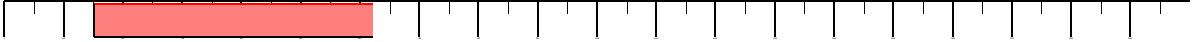
\includegraphics[scale=0.1]{chronogrames/4.jpeg}};
   \node (1) at (1,3){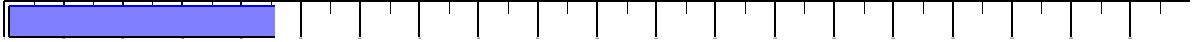
\includegraphics[scale=0.1]{chronogrames/1.jpeg}};
   \node (2) at (1,7){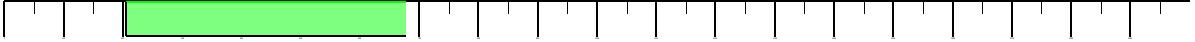
\includegraphics[scale=0.1]{chronogrames/5.jpeg}};
   \node (2) at (4,5){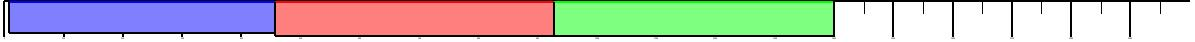
\includegraphics[scale=0.1]{chronogrames/6.jpeg}};
 \end{tikzpicture}
 }}}\\

This solution is optimal because the messages will not wait on source nodes, that is $\omega(r) = 0$, $\forall r \in \rho$. $T_{max}$ is
equal to twice the physical delay of the longest route, which is given in the input.\\


Following this observation, one can try to solve another problem for cases 2 and 3: is it possible to find a TwoWayTrip
with all $w_i = 0$ ? 

It is always possible when the period $P$ is large enough (for example: send all messages one by one, waiting for the previous one to be back),
therefore the problem is to find the smallest period such that it is possible.

\begin{subsection}{Star affectation}
 
Let us define a simplification of a matched graph. 
We start from a matched graph $N$ in which we forget weights on arcs starting from leaves, and the middle link.
We obtain a graph in which we have a central node, and different routes going to each sources.
Such a graph is called a {\bf star}.
The source Switch of $N$ is the central node $C$ of the star, and the source nodes $s_i$ of $N$ are kept. 
The weight of links between the sources switch and each $s_i$ in $N$, are the same in the star, denoted by $d_i$, where i is the number of the route in $\rho$. 
A ${\cal R}$-matching $\rho$ in a star is associating a route $r_i$ to a source node $s_i$.\\

\fbox{\parbox{11cm}{

\begin{center}

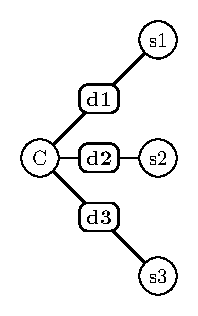
\includegraphics[scale=0.7]{Fig11.pdf}\\
Example of a star for a matched graph with 3 routes
\end{center}


}}\\


We can do this simplification of a matched graph N only if we search an affectation without waiting times: in this case, any solution
will be optimal, because the $T_{max}$ will be twice the delay of the longest route. So, a solution for a star, is a solution for a matched
graph, without waiting times. If waiting times are allowed, we are forced to consider the delay of the routes and this model is not
correct anymore.

A TwoWayTrip affectation of a matched-graph $N$ in which there is no waiting time, $\omega(r) = 0 \,\forall\, r \,\in\, \rho$ is a {\bf star affectation}.

In this simplified model, we have one parameter left: the travel time of each routes $2d_i$.
We have to set the beginning offsets $o_i$ such that a route have no collisions with the others, 
according to the definition of the collisions, given in Sect. \ref{topologiescases}.


We define a new problem: 


\noindent {\bf Star affectation (SA)} 

\noindent {\bf Input:} a star s, integer $P$.

\noindent {\bf Question:} does there exist a star affectation of s in a period $P$.\\

This is our main problem, but by finding the smallest $P$ for which there is a star affectation, we can know 
the minimal period given by our algorithm. The smallest the period is, the better is the algorithm.


\noindent {\bf Optimization goal:} minimizing $P$ .\\

In the case where we find a star affectation, it gives us an optimal solution for cases 2 and 3.
In the case where there is no solution without waiting times, there still can exist some solution with waiting times in 
a period $P$.
\end{subsection}
\begin{subsection}{Shortest Longest}
 
We suggest the following algorithm to find a star affectation in which $d_0$ is the shortest route, and $d_{{\cal L}-1}$ the longest one, 
${\cal L}$ is the number of routes and T is the size of the messages:

\begin{algorithm}[H]
\caption{Star affectation from shortest to longest}
\begin{algorithmic}

\REQUIRE star s
\ENSURE star affectation in $P \le {\cal L}*T + 2d_{{\cal L}-1} - 2d_0$
\STATE $offset \leftarrow 0$
\FORALL{routes i in $\rho$ from the shortest to the longest }
\STATE $o_i \leftarrow offset$
\STATE $offset \leftarrow offset+T$
\ENDFOR

\end{algorithmic}
\end{algorithm}


The message using the shortest route is sent before the others, so it come back to the central node before the others.
Recursively, the second message is sent before the others, and also will be back before the other messages. 
Because the second message is sent T slots after the first message ($o_2 = o_1 + T$, where T is the size of the message), it come back after
the end of the message one: $o_1+ T + 2a_1 \le o_2 + 2a_2$ with $a_2 \ge a_1$.

\paragraph{Period}
The period given by this algorithm is $P$ =${\cal L}$ * T + 2$(\lambda(r_{{\cal L}-1}) - \lambda(r_0))$, if routes $\{r_0,...,r_{{\cal L}-1}\}$ are ordered
from the shortest to the longest. 2$\lambda(r_0)$ is the first slot in which the first message is starting to pass through the sources switch,
and 2$\lambda(r_{{\cal L}-1})$ + ${\cal L}$ * T  is the time at which the last message has totally passed the switch.
Therefore, the period only depends of the difference between the longest and the shortest route: the larger this value is, the larger
the period is.

\paragraph{Complexity}
This algorithm runs in $O({\cal L}.\log({\cal L}))$. It represent the cost to sort the routes.
Indeed,once the routes have been sorted,the algorithm does a constant number of instruction for each route.
\end{subsection}

\begin{subsection}{Greedy Prime}

The following algorithm is a way to find a star affectation by a greedy way.

\begin{algorithm}[H]
\caption{Greedy Prime assignment}
\begin{algorithmic}
\REQUIRE star s, period $P$
\ENSURE star affectation in a period $\leq P$ 
\STATE $P1[P]$ slots in first way period.
\STATE $P2[P]$ slots in back way period.
\FORALL{route i in $\rho$ }

\FORALL{slot j in P1}

\IF{$[j,j+T]_P$ is free in P1}

\IF{$[j + 2d_j,j + 2d_j+T]_P$ is free in P2}

\STATE $o_i \leftarrow j$
\ENDIF

\ENDIF
\IF{No intervals are found for i}
\STATE return FAILURE
\ENDIF
\ENDFOR

\ENDFOR

\end{algorithmic}
\end{algorithm}


In this algorithm, for each route i, search for the first free slot [j,j+T] in P1 such that the slot $[j + 2d_i,j + 2d_i+T]$ in P2 is free too,
then give the route the offset j shifted by the distance from the leave to the first node.\\

We have no theoretical results on this algorithm, but after the experimental analysis, we will see that it is relatively good.


\paragraph{Complexity}
This algorithm runs in $O({\cal L}.P)$, where ${\cal L}$ is the number of routes. For each route, the algorithm tries the $P$ possible
starting slots and tests whether there is a collision on the way back.
The cost of testing if there is a collision between two message is constant because all the message have the same length. So we can easily know if an interval is free or not.

\end{subsection}




\begin{subsection}{Greedy Star}
%  
% 
% We can also use a greedy algorithm, choosing the offset of each packet in turn so that there is no collision. 
% We must chose an offset $o_i$ for each route $r_i$, so that no two routes have a collision when they return to central node.  
% We denote by $[o_i]_P$ the set of times $\{ t \mod P \mid o_i \geq t < o_i + T \}$ which are the time used by the route $r_i$ on the central
% link on its first use. There are no collision if for all $i\neq j$
%  $[o_i]_P \cap [o_j]_P = \emptyset$. Moreover no two routes must have a collision on the way back, hence we must have for all $i\neq j$
%  $[o_i + a_i]_P \cap [o_j + a_j]_P = \emptyset$.
%  
%  


This algorithm, looks like the Greedy Prime, in which the period in SL is divided in buckets of $\frac{P}{2T}$ slots. The period in SS is divided in $\frac{P}{T}$ slots.
For each route, search for a free bucket in P1, then set $o_i \in [j.2T,(j+1)2T]$ so that $o_i + d_i \mod P = kT$.
If $[kT,(k+1)T]$ is free, then allow the route to use the bucket $[j.2T,(j+1)2T]$ in the first period.\\



\begin{algorithm}[H]
\caption{Greedy Star assignment algorithm}
\begin{algorithmic}
\REQUIRE star s, period $P$
\ENSURE star affectation in a period $\leq $ $P$ 
\STATE $\frac{P}{2T}$ slots in first way period.
\STATE $\frac{P}{T}$ slots in back way period.
\FORALL{route i in $\rho$ }

\FORALL{slot j in P1}

\IF{P1[j] is free}

\STATE shift $\leftarrow$ T- 2$d_i \mod P$ 

\IF{The corresponding bucket in P2 is free}

\STATE $o_i \leftarrow 2Tj + shift$
\ENDIF

\ENDIF

\IF{No intervals are found for i}
\STATE return FAILURE
\ENDIF
\ENDFOR

\ENDFOR

\end{algorithmic}
\end{algorithm}


\paragraph{Period}
One can prove that if $P$ is large enough with regard to $\cal{L}$ and $T$, then there is always a TwoWayTrip
with waiting time $0$ with this algorithm.
 Assume $P \geq 4lT$, the algorithm works as follows. 
We cut the periods of size $P$ into $2\cal{L}$ slots of size $2T$ and we will asign one to each route.
A different slot is assigned to each route, where the offset is chosen inside the slot so that 
no collision on the first way in the central link is possible. If the slot chosen for the route $r_i$ is $[j2T,(j+1)2T]$,
then we set $o_i \in [j2T,(j+1)2T]$ so that $o_i + d_i \mod P = kT$. Assume that the offset of the first $i-1$ routes have been 
chosen in the previous way so that there is no collision. Since we have $P \geq 4lT$, we have at least $2\cal{L}-i$ possible choices of offset without collision on the first use of the central link. Each of these choices uses a time slot of size $T$ on the way back on the central link. Since there are $i$ time slots used, and $i \leq \cal{L}$, we have strictly more than $\cal{L}$ possible choices and less than $\cal{L}$ of them are forbidden, therefore there is a choice of offset with no collision. 
Since the algorithm works for all $i \leq \cal{L}$, it finds a TwoWayTrip with waiting times $0$. 

\paragraph{Complexity}
This algorithm runs in $O({\cal L} . \frac{P}{2T})$, where ${\cal L}$ is the number of routes.
This algorithm is the same than the Greedy Prime, but it uses buckets instead of the full period $P$.
\end{subsection}


\begin{subsection}{Exhaustive Generation}
 To try finding a solution without waiting times, we tried to implement a naive algorithm testing all the different starting offsets.
 Such an algorithm was just too slow: indeed the number of possible instances is exponential. With a period of 20000 slots,
 and 7 routes, we have over $10^{28}$ possibilities which is not practically computable.
 The following algorithm is a ''smart bruteforce``, an exhaustive generation of the possibilities with heuristics.
 
\begin{algorithm}[H]
\caption{Exhaustive Generation}
\begin{algorithmic}
\REQUIRE Matched graph N, period $P$, packet size T
\ENSURE 2way Trip affectation in P
\STATE BUDGET $\leftarrow$ $P$ - ${\cal L}$ * T
\STATE offset $\leftarrow$ 0
\FORALL{route i in $\rho$ }
\FORALL{j from offset to offset + BUDGET }
\IF{Message of the route i does not collides with other routes, and some conditions are observed}
\STATE Give i the offset j
\STATE BUDGET $\leftarrow$ BUDGET - (j - offset)
\STATE offset $\leftarrow$ j
\STATE call Exhaustive Generation on remaining routes
\ENDIF
\ENDFOR
\ENDFOR


\end{algorithmic}
\end{algorithm}

This algorithm enumerates all the solutions by traversing a tree. The leaves of the tree are 
the TwoWayTrips without waiting times, and the nodes are partial solutions. A partial solution is a choice of a starting time for a subset of the routes.
For each route, the algorithm tries every possible starting offset until it finds one available (that allows the message to come back without collisions). When a route have been scheduled, it take another route that have not been scheduled yet.
This creates a new sub-tree in which the algorithm will try every possible starting offset too, and create a sub-tree on the following route too.
If no offset are available for a route, this means that the partial solution is not good, so the algorithm backtracks over the tree that is,
it goes back to the father of the current sub-tree.
Once a leaf is obtained, the algorithm stops and return the scheduling.

We have implemented cuts so the algorithm avoids to browse some parts of the tree that will not give any solution.
\begin{enumerate}
 \item The budget: It is the number of slots that can be wasted in the first period. If this budget comes below 0, then the period is too small with regard to
 the solution.
 \item When a starting offset is given to a route, the interval used by the route on the source's switch is also set. If there are less than T slots
 between the end of the previous message and the beginning of the actual message, then no future messages can be scheduled in this gap.
 So, if the solution isn't found with the first offset, the algorithm will directly skip to the offset corresponding to a gap of T slots.
 \item There is also a budget for the second period. When a message is put on the way back period, there is a possibility that its position definitively block the place for an other message. For example, if a message is put in a gap of 3 possible messages, but in a position such that there is only the space for 0.5 of a message before and 1.5 after. Then, the number of possible messages in this gap of 3 messages is now 2 and the message has burned 2 slots, one for itself and one by its positioning.
 Once this number of possible messages has reached 0, the algorithm backtrack.
\end{enumerate}

Because of the cuts, one can hope that this algorithm which has an exponential complexity works fast enough to find a solution with our settings.

\end{subsection}

 \end{section}

\begin{section}{Finding a TwoWayTrip with waiting times}
\begin{subsection}{Waiting times are useful}
 
The following example shows us that you can find a TwoWayTrip affectation such that there is no waiting time, but it needs a greater period $P$ than a
solution with waiting times.

Consider the graph: 
\begin{center}
 
\fbox{\parbox{11cm}{  
\scalebox{0.6}{
\begin{tikzpicture}
  \SetGraphUnit{5}
  \Vertex[x=0,y=0]{l1}
  \Vertex[x=0,y=4]{l2}

  
  \Vertex[x=16,y=0]{s1}
  \Vertex[x=16,y=4]{s2}

  \Vertex[x=4,y=2]{SL}
  \Vertex[x=12,y=2]{SS}
  

  \tikzset{
  EdgeStyle/.append style = {red} }
  \Edge[label = 1](s1)(SS)
  \Edge[label = 10](SL)(l1)
  
  \tikzset{
  EdgeStyle/.append style = {green} }
  \Edge[label = 10](s2)(SS)
  \Edge[label = 1](SL)(l2)
  
  
  \tikzset{
  EdgeStyle/.append style = {black} }
  \Edge(SL)(SS)
\end{tikzpicture}
  }}}\\
\end{center}

Consider messages of 10 slots. If you search for a $P$-periodic affectation, without using waiting times, there are 2 choices: 
\begin{itemize}
 \item l1 is sent before l2: the message from l1 will leave A after 11 slots. X is he minimal time slot in which l2 can emit. 
 To avoid collisions with the message from l1 in A,l2 must emit after 1 slot:  $X\ge1$.
 In the other way, the message from l1 will use B from time slot 21 to 30. The route from l2 is 12 units long from l2 to B. So, to avoid collisions with 
 the message from l1 in B $X+12 \ge 31 \rightarrow x\ge 19$. Then, by taking $X=19$, the time
 The period is at least 38 slots in A (corresponding to the transit time of the 2 messages and the time lost between those 2 transits).
 \item l2 is sent before l1: symmetrically the collision occurs in node A if l1 emits before time 19. The period in B is at least 38 too.
\end{itemize}

\fbox{\parbox{11cm}{
\scalebox{0.6}{
  
\begin{tikzpicture}
  \SetGraphUnit{5}

  
  \node (0) at (1,-1){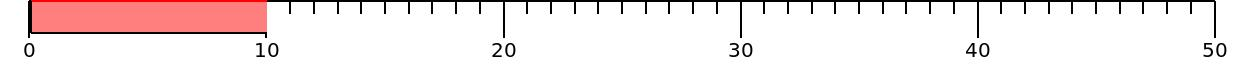
\includegraphics[scale=0.1]{chronogrames/10.jpeg}};
  \node (1) at (1,5){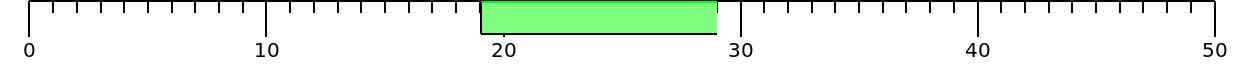
\includegraphics[scale=0.1]{chronogrames/11.jpeg}};
  \node (2) at (5,2){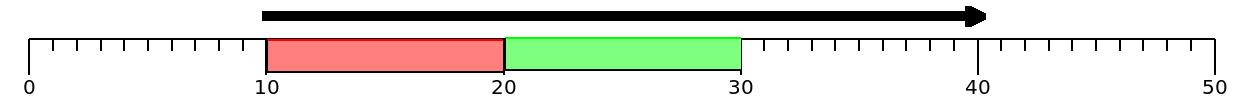
\includegraphics[scale=0.1]{chronogrames/12.jpeg}};
  \node (3) at (10,2){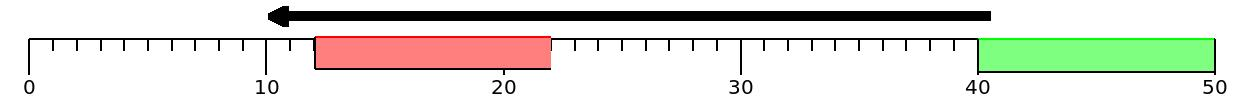
\includegraphics[scale=0.1]{chronogrames/15.jpeg}};
  \node (4) at (15,-1){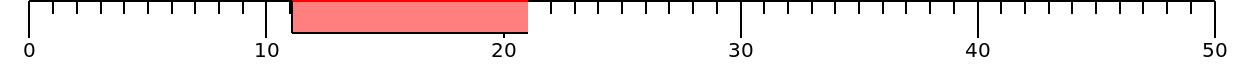
\includegraphics[scale=0.1]{chronogrames/13.jpeg}};
  \node (5) at (15,5){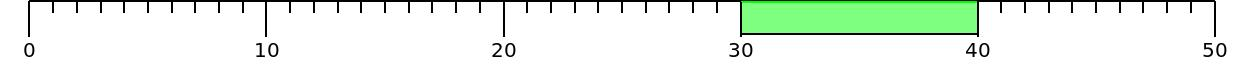
\includegraphics[scale=0.1]{chronogrames/14.jpeg}};
  
     \Edge(2)(3)
    \tikzset{
    EdgeStyle/.append style = {red} }
    \Edge[label = 10](0)(2) 
    \Edge[label = 1](3)(4)

    \tikzset{
    EdgeStyle/.append style = {green} }
    \Edge[label = 1](1)(2)
    \Edge[label = 10](3)(5)
\end{tikzpicture}
  } 
  Without waiting times: period of 38(2k + 18) slots, $T_{max}$ = 22 slots.
  }}\\
 


If we allow waiting times: there is an easy scheduling using only a 3 time slots period: 
Sending message 1 at time 0, message 2 at time 1, so the messages will not cross A in the same time. to be sent back,
message 2 comes back immediately and is using B from slots 13 to 22,then message 1 is using B from slots 23 to 32, waiting 2 time slots at s1.

So the smaller periods is 20, half smaller than the best solution without waiting times.\\

\fbox{\parbox{11cm}{
 \scalebox{0.6}{
  \begin{tikzpicture}
  \SetGraphUnit{5}

  
  \node (0) at (1,-1){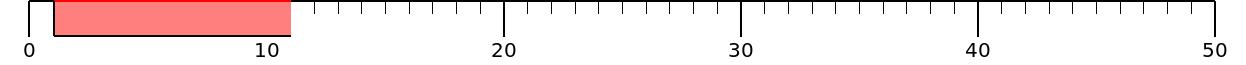
\includegraphics[scale=0.1]{chronogrames/22.jpeg}};
  \node (1) at (1,5){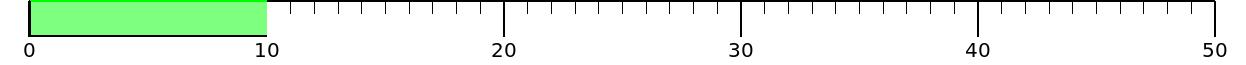
\includegraphics[scale=0.1]{chronogrames/21.jpeg}};
  \node (2) at (5,2){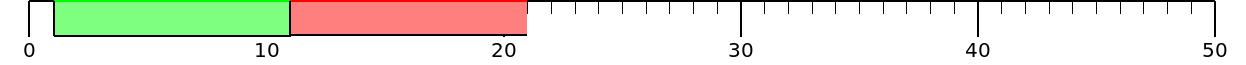
\includegraphics[scale=0.1]{chronogrames/23.jpeg}};
  \node (3) at (10,2){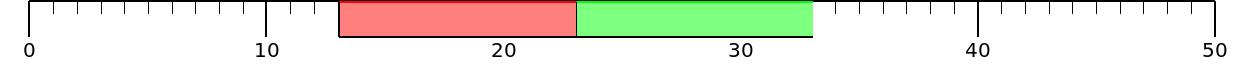
\includegraphics[scale=0.1]{chronogrames/26.jpeg}};
  \node (4) at (15,-1){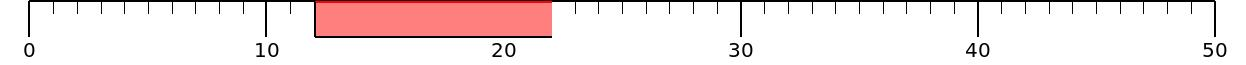
\includegraphics[scale=0.1]{chronogrames/25.jpeg}};
  \node (5) at (15,5){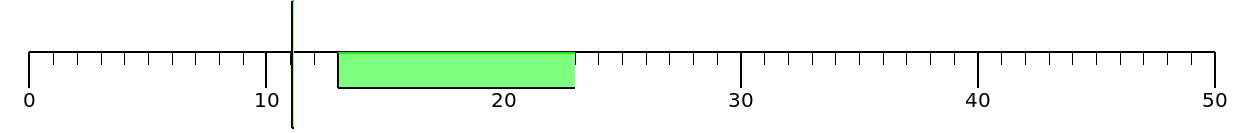
\includegraphics[scale=0.1]{chronogrames/24.jpeg}};
  
     \Edge(2)(3)
    \tikzset{
    EdgeStyle/.append style = {red} }
    \Edge[label = 10](0)(2) 
    \Edge[label = 1](3)(4)

    \tikzset{
    EdgeStyle/.append style = {green} }
    \Edge[label = 1](1)(2)
    \Edge[label = 10](3)(5)
\end{tikzpicture}
  }
  
    With waiting times: period of 20(2k) slots, $T_{max}$ = 24 slots.

  }}\\
  
  Allowing the waiting times gave us the possibility to reduce the period from 38 slots to 20, with only 2 times slots added to $T_{max}$.
\end{subsection}
\begin{subsection}{Longest Shortest + Greedy}
 

To find a solution allowing waiting times, the following heuristic is suggested:

On leaves switch, the messages are scheduled so that they are following each others, from the one using the longest route, to the one using the shortest route.

On sources switch, the politic is the following one, after setting the clock to 0, do:
\begin{enumerate}
 \item To be eligible, a job needs to be able to come back on the switch at the current clock (if clock = 0, take the first message able to come back).
 \item Between the eligible jobs, schedule first the one which has the longest route gives it the starting time $o_i = clock$.
 \item Update the clock at the time in which the scheduled task is over: $$clock = clock + message_length$$.
\end{enumerate}

This algorithm defines the offsets of the first $P$-periodic affectation by sending the messages from the longest route to the shortest route, then it uses a greedy algorithm to schedule the messages in the second $P$-periodic affectation. We denote this algorithm by LSG (Longest Shortest + Greedy).

\begin{algorithm}[H]
\caption{LSG}
\begin{algorithmic}
\REQUIRE Matched graph N, period $P$, packet size T
\ENSURE 2way Trip affectation in P
\STATE clock $\leftarrow$ 0
\FORALL{route i in $\rho$ from the longest to the shortest }
\STATE  $m_i \leftarrow$ clock
\STATE clock $\leftarrow$ clock + T
\ENDFOR
\STATE clock $\leftarrow$ 0
\STATE take i such that $r_i$ is the first route to come back in sources switch
\STATE $o_i \leftarrow $ clock;
\STATE clock $\leftarrow$ $a_i$ + T
\WHILE{there is a route which has no $w_i$}
\STATE take i such that $r_i$ is the eligible route.
\STATE $o_i \leftarrow $ clock - $a_i$;
\STATE clock $\leftarrow$ clock + T

\ENDWHILE

\end{algorithmic}
\end{algorithm}


\paragraph{Period}
This algorithm gives us solution with a small period. Indeed, we have not studied the period given by this algorithm but we can imagine that ${\cal L}$ x T + C will not explode. C is a constant representing of the slots wasted when no routes are eligible.
We can obtain the minimum possible period: ${\cal L}$ x T, by choosing the route $r_i$ having the longest arc SS-$s_i$ on the second part of the heuristic, instead of choosing the route having the longest total length of route. Indeed with such a policy all the messages are scheduled following each others on switches and there is no wasted time between the transit of two messages.
This variation of our algorithm gives us a better period but could also gives us some poorer results.

\paragraph{Analysis}
For the case 1, this algorithm is similar to the obvious way to schedule the messages mentioned above. It gives an optimal solution without increasing 
the computation time.

For the case 2, this algorithm gives optimal solutions: Indeed, in the manner we order messages, from leaves toward sources,
the messages are sent from the one using the longest route to the one using the shortest one. Number the routes in this order from 1 to ${\cal L}$.

We have $\forall \ i<j$, $r_i<r_j$.
The first message leaves the source switch at time 2$r_1+T$, the second message, can use it at the time 2$r_2+T$.
The second message waited $2r_1+T-(2r_2+T) = 2(r_1-r_2)$ to use the middle link. So, the second message leave the source switch at time
2$r_2+T + 2(r_1-r_2) = 2r_1 +T$.
By induction, all messages will take $2r_1 +T$ slots for the TwoWayTrip.
Consequently, for this case, the heuristic is optimal, because the longest route has no waiting time and no TwoWayTrip is longer than the longest route one.

We have no guarantee for the case 3. We can not say if this algorithm gives an optimal solution for any values on all arcs, but we think that on parameters corresponding to the realistic problem, the solutions given by LSG are good.Indeed the experimental study of the following chapter shows such a behaviour.

\paragraph{Complexity}
By using a binary heap to implement a priority queue to store the eligible routes, this algorithm runs in $O(n.\log(n))$, 
where n is the number of routes. For each route, there is a deletion and an insertion in the heap.
\end{subsection}

\begin{subsection}{Longest Shortest + Optimal}
 The algorithm studied in Barbara Simons's article \cite{simons1978fast} gives us an improvement of the Longest Shortest algorithm.
 \begin{algorithm}[H]
\caption{LSO}
\begin{algorithmic}
\REQUIRE Set of tasks S
\ENSURE Scheduling in a minimal time.
\STATE CLOCK $\leftarrow$ 0
\WHILE{ S $\ne \emptyset$}
\STATE Select X the not scheduled job with the lower deadline in the eligible jobs
\IF{X has a CRISIS}
\STATE call CRISIS(X)
\STATE CLOCK = end of the returned restricted set
\ELSE
\STATE CLOCK += task-length
\ENDIF

\ENDWHILE

\end{algorithmic}
\end{algorithm}
As a reminder, a job is eligible if its release date is lower or equal to the actual clock. If no such a job exists, the eligible job is the one
with the lowest release time.

 \begin{algorithm}[H]
\caption{Crisis Subroutine}
\begin{algorithmic}
\REQUIRE A crisis job X
\ENSURE New scheduled r.s.
\STATE backtrack over the scheduling and find PULL(X)
\IF{ PULL(x) $= \emptyset$}
\STATE Exit Failure
\ENDIF 
\STATE Remove and count the jobs in each interval between the inner restricted sets
\STATE Increase the initial interval number by 1
\WHILE{Some jobs have not been scheduled}
\STATE Use the naive algorithm to schedule the required number of jobs in each interval.
\IF{Some job X has a CRISIS}
\STATE Call CRISIS(X)
\ELSE
\IF{Some job Y invades the following r.s. S'}
\STATE call INVASION(S', $t_{S'}$)
\ENDIF
\ENDIF
\ENDWHILE

\end{algorithmic}
\end{algorithm}
$t_{S'}$ is the time at which the job Y is completed.


 \begin{algorithm}[H]
\caption{INVASION Subroutine}
\begin{algorithmic}
\REQUIRE S' a r.s., $t_{S'}$ a begin date.
\ENSURE New scheduled r.s.
\STATE Remove and count the jobs in each interval between the inner restricted sets
\WHILE{Some jobs have not been scheduled}
\STATE Use the naive algorithm to schedule the required number of jobs in each interval.
\IF{Some job X has a CRISIS}
\STATE Call CRISIS(X)
\ELSE
\IF{Some job Y invades the following r.s. S'}
\STATE call INVADE(S', $t_{S'}$)
\ENDIF
\ENDIF
\ENDWHILE

\end{algorithmic}
\end{algorithm}


A job $A$ has a release time $r_A$, a deadline $d_A$, and a schedule time $t_A$. The jobs have the same running time $p$.
The running of this algorithm is the following one:
The main algorithm starts to schedule the jobs by the following rules:

\begin{enumerate}
 \item To be eligible, a job needs to have a release time lower or equal to the current clock.
 \item Between the eligible jobs, schedule first the one which has the lowest deadline; give this job the time $t_A = CLOCK$
 \item Update the clock at the time in which the scheduled task is over.
\end{enumerate}
At this moment, this algorithm is exactly the same than the greedy part of LSG. The following subroutines are an improvement of the greedy part, and the reason why the second $P$-periodic affectation of the TwoWayTrip given by LSO is optimal.\\


If a selected job (let us call it X) has an insufficient time to run ($t_A + p > d_A$), then X is a CRISIS job.

The Crisis subroutine is called when there is a crisis job. It searches through the schedule starting at the end,
and tries to find a job with an higher deadline.
If such a job exists, it is called PULL(X). Otherwise, the algorithm fails.
Let us call PULL(X) A.
All the browsed tasks from X(included) to A(excluded) are forming a new set called restricted set S(A,X].
The algorithm tries to reschedule the jobs in S(A,X] by the main algorithm rules, if another crisis occurs, the crisis subroutine recursively calls
itself.

In case of the crisis subroutine is backtracking over a restricted set, it does not reschedule this r.s.. The subroutine only counts
the number of jobs between the r.s. and reschedule exactly the same number of jobs after the backtracking.

During this rescheduling, some jobs may overlap an r.s.. In this situation, the subroutine INVASION is called on this r.s..

The Invasion subroutine just counts the number of jobs between the intervals of the r.s. and reschedule the jobs with the new starting time,
which correspond to the completion time of the task before the r.s..



\paragraph{Complexity}
This algorithm runs in $O(n^2 \log(n))$, where n is the number of tasks. This complexity is given by the author of the article, based on the fact that a task can crisis only once.

\paragraph{Adaptation to our problem}
This algorithm allows us to improve the second $P$-periodic affectation of the Longest Shortest algorithm. 
Indeed, it yield, in polynomial time, an optimal solution with a given set of jobs with release times and deadline. 
In our adaptation, we choose by the greedy way of LSG the first $P$-periodic affectation that gives us the release times and deadlines. Then, the algorithm ensure us to find the optimal second $P$-periodic affectation, for these release times and deadlines
Because we arbitrarily chose the first $P$-periodic affectation, the problem is not solved.

We set the first $P$-periodic affectation by using the same politic than LSG. This $P$-periodic affectation gives us, for each route, the time in which the message will be able to be in the sources switch. This is the release time of the messages. Then, we set the deadlines of the messages by choosing the minimum between two values: 
\begin{enumerate}
 \item The time in which the first message came back on sources switch + P-T.
 \item The maximum delay allowed - the physical transit time of the route.
\end{enumerate}

The first value ensure us to have a periodic process of period $P$. The second corresponds to the first constraint of the problem: to not exceed a deadline.\\
This algorithm allows us to have an optimal second $P$-periodic affectation of the TwoWayTrip. For the first $P$-periodic affectation, we still send the route in the same manner as in LSG: from the longest route to the shortest. That is why is algorithm is called LSO(Longest Shortest + Optimal).


\end{subsection}

\end{section}

\end{chapter}

\begin{chapter}{Performance Evaluation}

In this chapter, we will try the previous algorithms on some instances of the topology 1.

\begin{section}{Real values}
 The experiences are made on values corresponding the real situation.
  
  The time of a period is 1ms and the maximum delay of a TwoWayTrip is 3ms. The computation time is 2.6ms, so the deadline is 0.4 ms.
  
 The topology 1 that we are studying correspond to a maximum range of 5km, the links have a bandwidth of 10Gb/s and the flows are of 1.228Gb/s.
 In time slots, this values correspond respectively to about 2100 slots on links, a period of 19500 slots and a flow of 2500 slots every ms.
 
 The graphs are randomly generated. The length of the routes is between 0 and 2100. More precisely
 each link of a path is generated following an uniform law between 0 and 700.
 
 \centering
  \begin{tabular}{|c|c|c|}
  \hline
   Links capacity & 10Gbp/s & -\\
   \hline
   Flow/RRH & 1.228Gbp/s & $\simeq$ 2558 slots/ms\\
   \hline
   Flow max ($l_{max}$) & 7 & -\\
   \hline
   Considered Range & 0-5km & $\simeq$ 2100 slots\\
   \hline
   Periodicity & 1ms & $\simeq$ 19500 slots\\
   \hline
   \end{tabular}
  
Each of this algorithm runs in a fraction of a second. The scheduling of a fronthaul network is computed once and does not 
need to be recomputed frequently. Thus, we did not mention the time taken to do each experiment on the study of the speed of the algorithms.
\end{section}

\begin{section}{No waiting time involve bigger periods}
First, let us study the algorithms trying to find solutions without waiting times.
We generated 10000 graphs and studied which algorithm finds a solution in the shortest period. We made and average of all the periods obtained for each algorithms
between The Greedy Star, The Greedy Prime, Shortest Longest and the Exhaustive Generation.
To find the minimal period in which the algorithms can find a solution, we made a linear search on the period. As explained above in Sect. \ref{slottedtime}, the notion of $P$-periodic affectation is not monotone with regard to $P$,  therefore we could not have done a dichotomous search on the period $P$.

The blue line is the lower bound of the period. The red one is an indication of 2 * ${\cal L}$ * T, T is the size of a message and ${\cal L}$ the number of flows.
\begin{figure}[H]
\hspace*{-3cm}
\centering
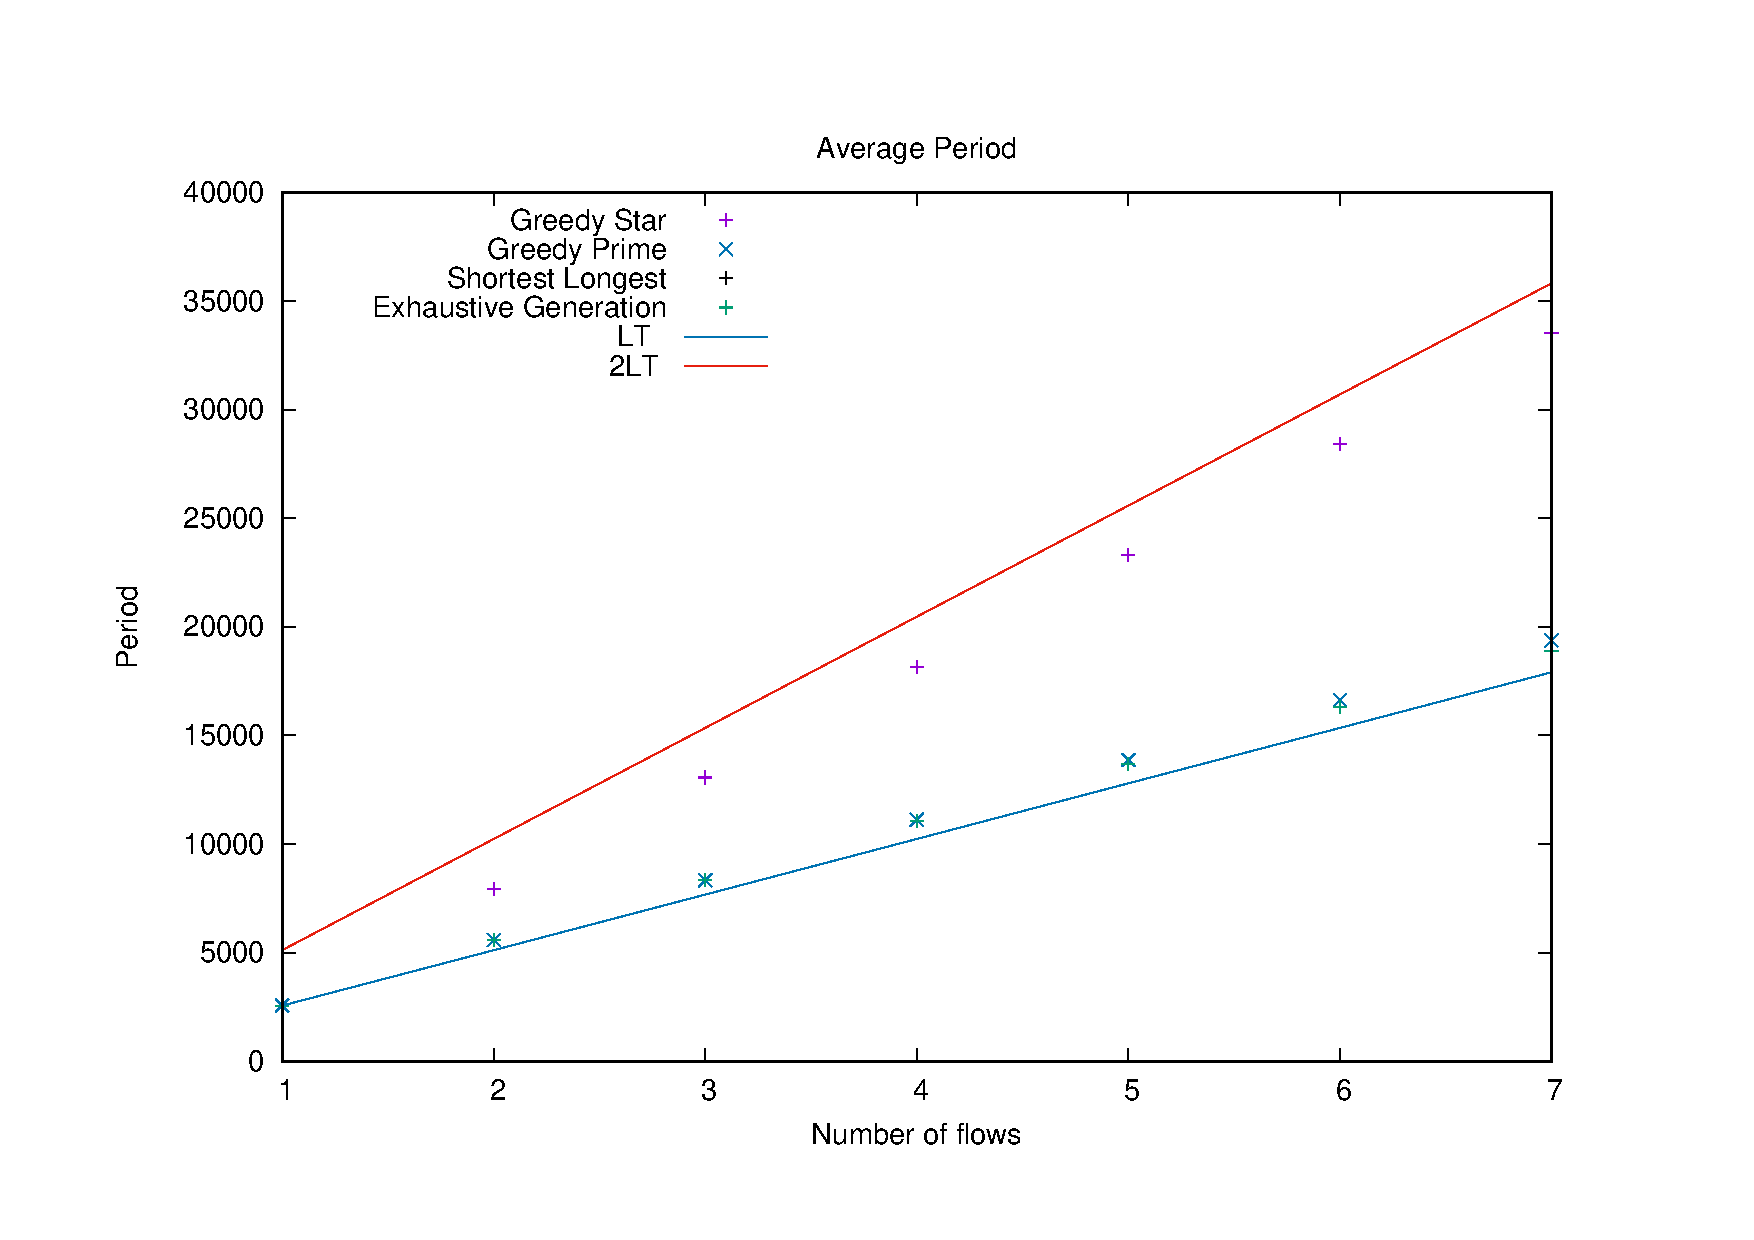
\includegraphics[scale=0.6]{window0.pdf}%scale=0.6
\caption{Average periods for algorithms without waiting times}
\end{figure}


Even if it has theoretical guarantee, the Greedy Star is not giving good solutions, as we can see, the average period for this algorithm is 
significantly higher compared to the others.

We observe that the Greedy Prime, the Shortest Longest and the Exhaustive Generation find some solution with very similar average periods.

The Greedy Prime gives us the worst solutions of the three algorithms. We did not expect it to be better than the Exhaustive Generation, but the fact that it is a greedy algorithm interested us for its simplicity and low complexity.
Even if the average period given by it is not that high compared to Shortest Longest or Exhaustive Generation, it is never advantageous to use the Greedy Prime instead of one of the two others, because it will not give a better solution.
The period given by the Shortest longest is known and depends of the difference between the longest and the shortest route.
In our context, this difference is never big enough to obtain bad periods. This algorithm is good in our context, however, if we allow the 
route length to be larger, the period could significantly increase.

The Exhaustive Generation algorithm finds some solutions in an average period very close to the lower bound.
On this figure, we observe that the Exhaustive Generation and the Shortest Longest are giving exactly the same average periods.
We did not theoretically proved that the Shortest Longest gives optimal solutions, but this experimental study suggests it does, on these parameters. This is probably due to the fact that the routes are shorter than the messages length.

% So, with our parameter, the two algorithms are giving the same average periods, but one can imagine that if we allow the routes to be longer, the Shortest Longest will give some solution with an higher average period than the Exhaustive Generation.

The conclusions are the same if we study the worst period needed on the 10000 experiences to find a solution without waiting times (cf Appendix Fig 1).
\end{section}

\begin{section}{Limits of avoiding waiting times}
Too see in which circumstances finding a solution without waiting times is reasonable, we progressively increased the load of a network,
then we looked how many times the Exhaustive Generation algorithm is finding a solution for each flows.
We made this experience on a network composed of 7 flows max, on a period of 19500 slots.
In a first time on a simulation of 10000 experiences, we observed that the success rate is always 100\%. This means that the Exhaustive Generation always finds a solution without waiting time on graphs with our parameters.
We can complicate a bit the model, and consider that the computation times are not the same on all routes. 
In this case, we would not simplify all the computation times and express it on the route lengths.
Thus, with a minor variation of this computation time, even 10\%, we could have some route increasing significantly their length. 
The following tabular is the result of 10000 experiences on a graph with the weight of the arcs of the star generated between 0 and 1660 ($\simeq$ 2.3 longer).

 \centering
  \begin{tabular}{|c|c|c|c|}
  \hline
   Number of flows & 1-5 & 6 & 7\\
   \hline
   Success(\%) & 100 & 66 & 0\\
   \hline
   \end{tabular}
   
   
As we can see, when the period is large enough according to the load, there is no problems. Nevertheless, when we the load exceeds a certain limit 
, here, 6 routes, the number of found solution decrease significantly, and fall to 0 with 7 routes.

In this situation, we have to find other options to find a solution. This is why we imagined some algorithm using the waiting times to delay some routes.

\end{section}

\begin{section}{LSG}

As we just noticed, it is not always possible to find a solution where the messages never wait anywhere in a given period.
LSG allows us to find some solution in the smallest possible period (L*T), but does this algorithm ensures a good maximum delay?
Does this algorithm improve significantly on actual way to manage the messages through a network ?

\begin{subsection}{LSO and LSG}

After the adaptation of the LSO to our problem, we realised that this algorithm is not useful for the parameters on which we use it. 

Indeed, once the first $P$-periodic affectation is chosen
by the algorithm, we have a set of tasks with release times and deadlines that does not trigger any crisis.
The release times and deadlines are regularly spaced in the time (ex: (1400-7000), (3900,9500), (9000,15000) ...).
This observation is due to the small size of our routes compared to the size of our messages. Then, when a message is sent, it arrive on sources switch before having totally passed the leave switch. Thus, there is no chance that an other message which have leave its leaf later arrive in sources switch before.
The algorithm will so take the tasks by their arrival order and send it back in the same order. If, however a crisis occurs, no tasks could be the PULL
of another one. By definition, a task can be the pull of another one, if and only if it has an earlier release time and a greater deadline, with this configuration, such a task does not exists.

Furthermore, LSO can fail if the routes are too long. Indeed, the deadlines are calculated according to the physical deadline. If we lengthen the routes, we decrease the deadline, then it is possible to have a task for which the time between the deadline and the release time would be inferior to T.
Nevertheless, with an high deadline, LSO tries to optimise the scheduling, and finds a the best scheduling, however the deadline, exactly like LSG.
In this case in which the deadline is high, the problem mentioned above about the fact that LSO never crisis is still the same. So LSO and LSG will still give the sames results.

We made some simulation on 10000 graphs generated by the same way than in the previous section.
On those graphs, we applied LSG and LSO, then we looked at the average and worst $T_{max}$.
As a reminder, $T_{max}$ is the longest time taken by a message to do the TwoWayTrip ( physical delay + waiting time).

As we can see in the Appendix Fig 2 and Fig 3, the results are strictly the same for the two algorithms. This is not surprising given the
theoretical explanations.
To see some different results between LSO and LSG, we could try to find some TwoWayTrip affectations on graphs with longer route.

Therefore, in the rest of the study, we talk only about LSG.
\end{subsection}


\begin{subsection}{Random against LSG}

Presently, the major part of the messages in a network are not really controlled: A message is sent and if it does not reach the destination,
it is re-sent until it is transmitted without loss. If many messages are crossing the same switch in the same time, some of them are buffered,
others are redirected or destroyed. This way to manage the messages is maladjusted to our problem in which the latency constraints are strong.

Thus, we compared our results on the LSG simulation with a random sending order, generated with the following laws: 
\begin{enumerate}
 \item The starting offsets are randomly generated, following a uniform law between 0 and P.
 \item If several messages are crossing the same switch at the same time, the first message passes and the others are buffered by arrival order, and sent as soon as possible.
\end{enumerate}

Then, we count the time for the messages to make the TwoWayTrip.\\
 
The following result shows us the difference of the average $T_{max}$ between our algorithm (LSG) and the current way to manage message in a network, modelled by the random sending.
The orange points represent the random sending results, and the black points represent the LSO results.
The blue circle are a bound i.e. the average size of twice the longest route in the generated graphs.
Indeed, this size is the physical delay of the longest route.
By definition, $T_{max} = \max_r T(r) \geq 2\lambda(r_i)$.
Thus, if $T_{max} = 2\lambda(r_i)$  that means the solution is optimal.

The red line is the deadline. It represents the 0.4 ms maximum for a message to do the TwoWayTrip.

\begin{figure}[H]
\hspace*{-3cm}
\centering
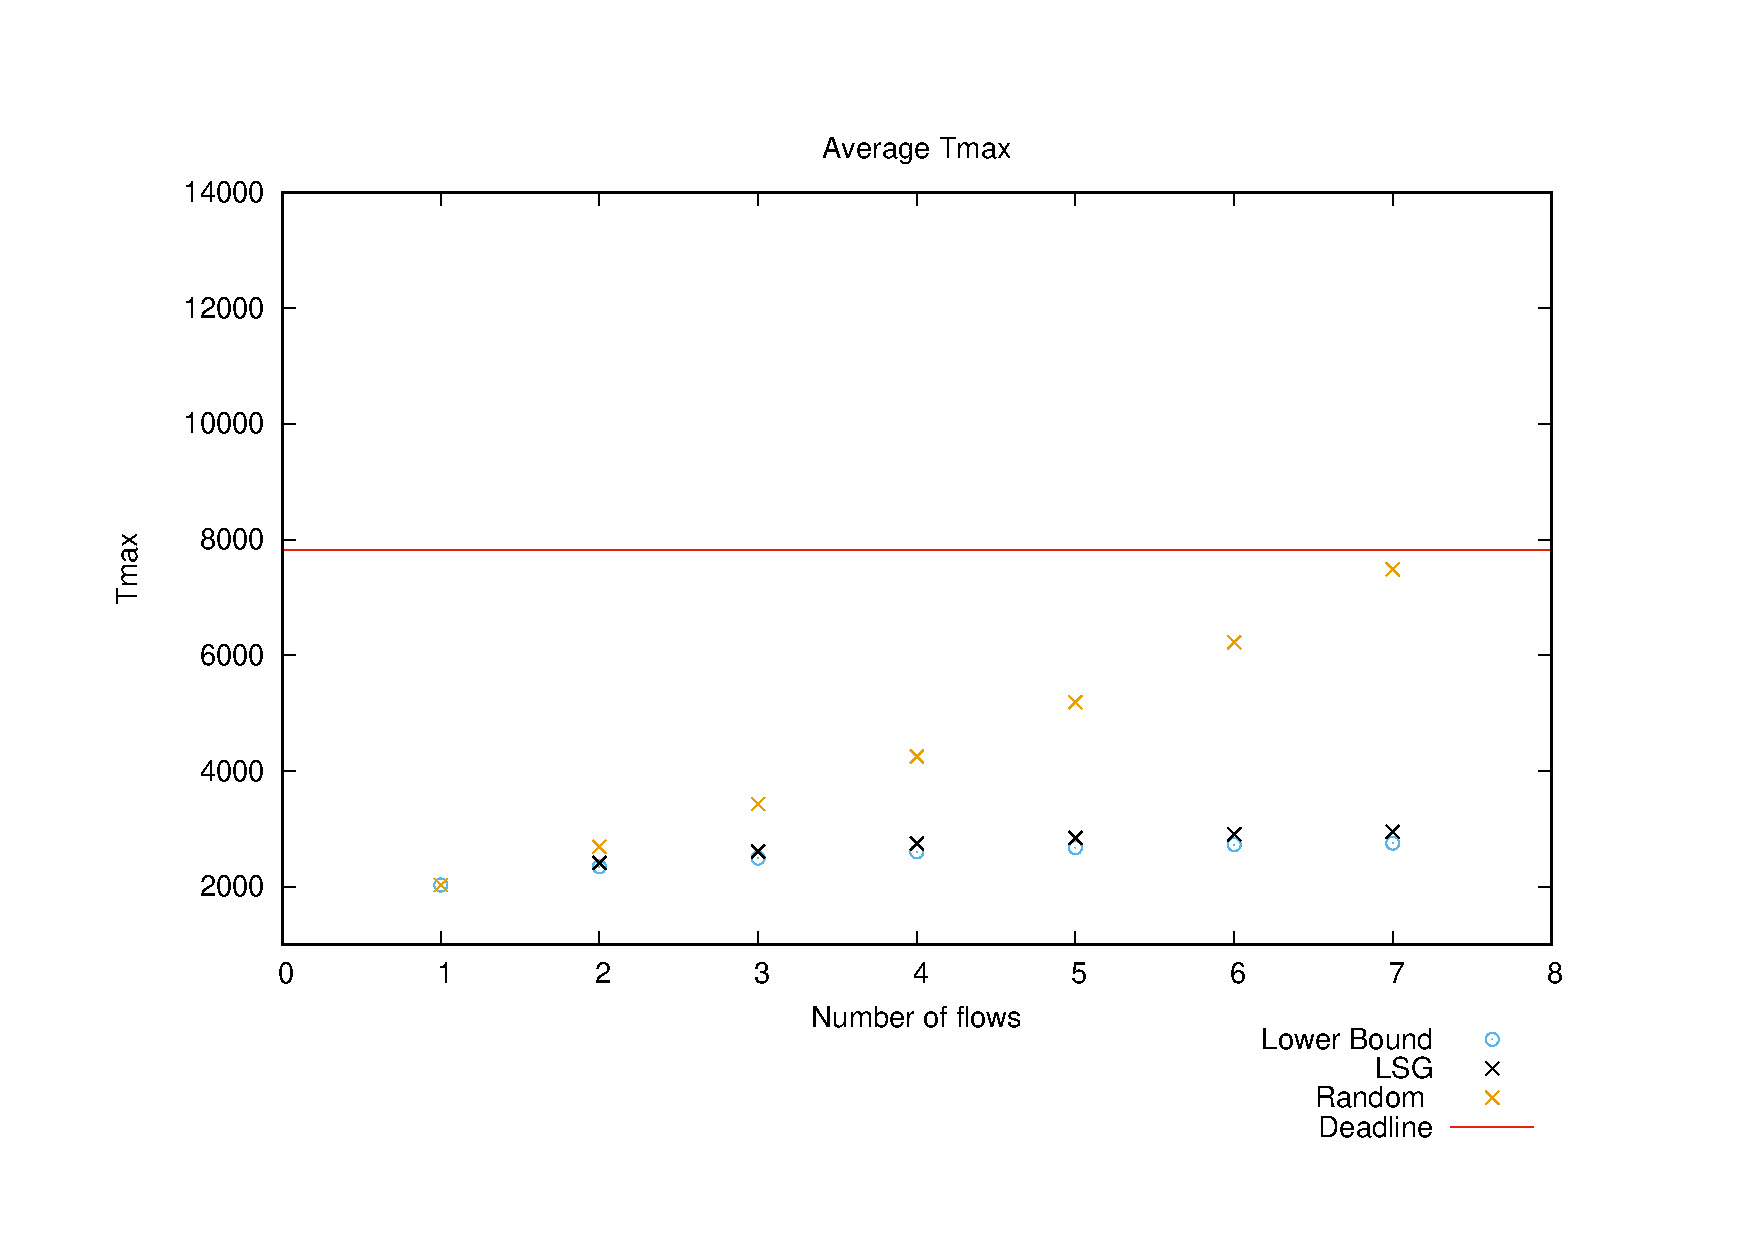
\includegraphics[scale=0.6]{tmax0.pdf}%scale=0.6
\caption{Average $T_{max}$ for the random sending and LSG deterministic sending.}
\end{figure}

LSG gives us some good results, close to the lower bound. On the other hand, for the random sending, 
the greater the load of the network is, the greater the average $T_{max}$ are. When the network starts to be congested, the 
message managing policy generates a lot of latency because of the buffering, so $T_{max}$ significantly increases, until the deadline for 5 flows or more.


Moreover, the worst case shows us that with LSG, $T_{max}$ never exceeds the deadline, while with the random sending, we already obtain some bad cases where $T_{max} > $ deadline when the load is equal to 3 flows (Cf Appendix Fig 4).


The two following figures show us the distribution of the $T_{max}$ on 100 000 graphs using first LSG, then the
random sending.
Each curve represents the distribution of $T_{max}$ for a given number of flows.
\begin{figure}[H]
\hspace*{-4cm}
\centering
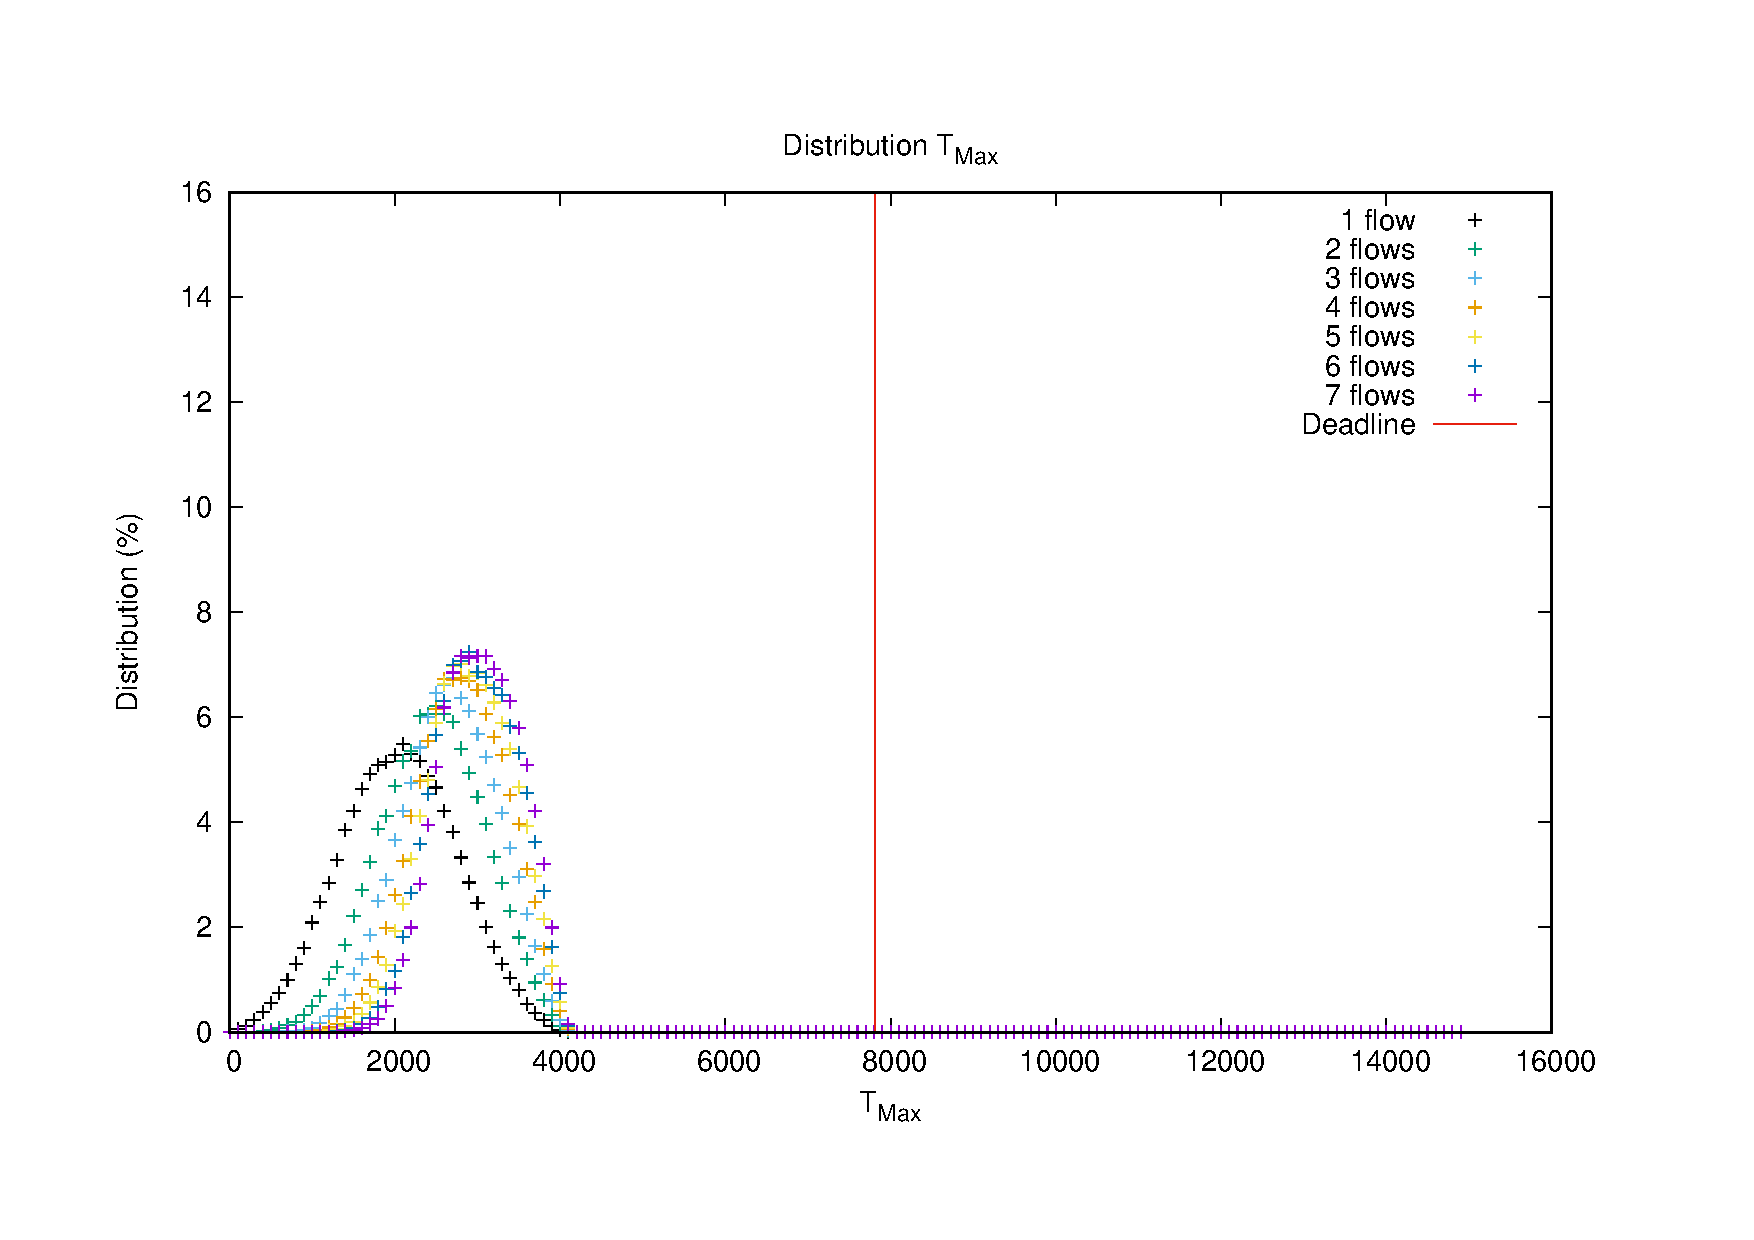
\includegraphics[scale=0.7]{distributions_longest.pdf}%scale=0.6
\caption{Distributions for LSG}
\end{figure}

\begin{figure}[H]
\hspace*{-3cm}
\centering
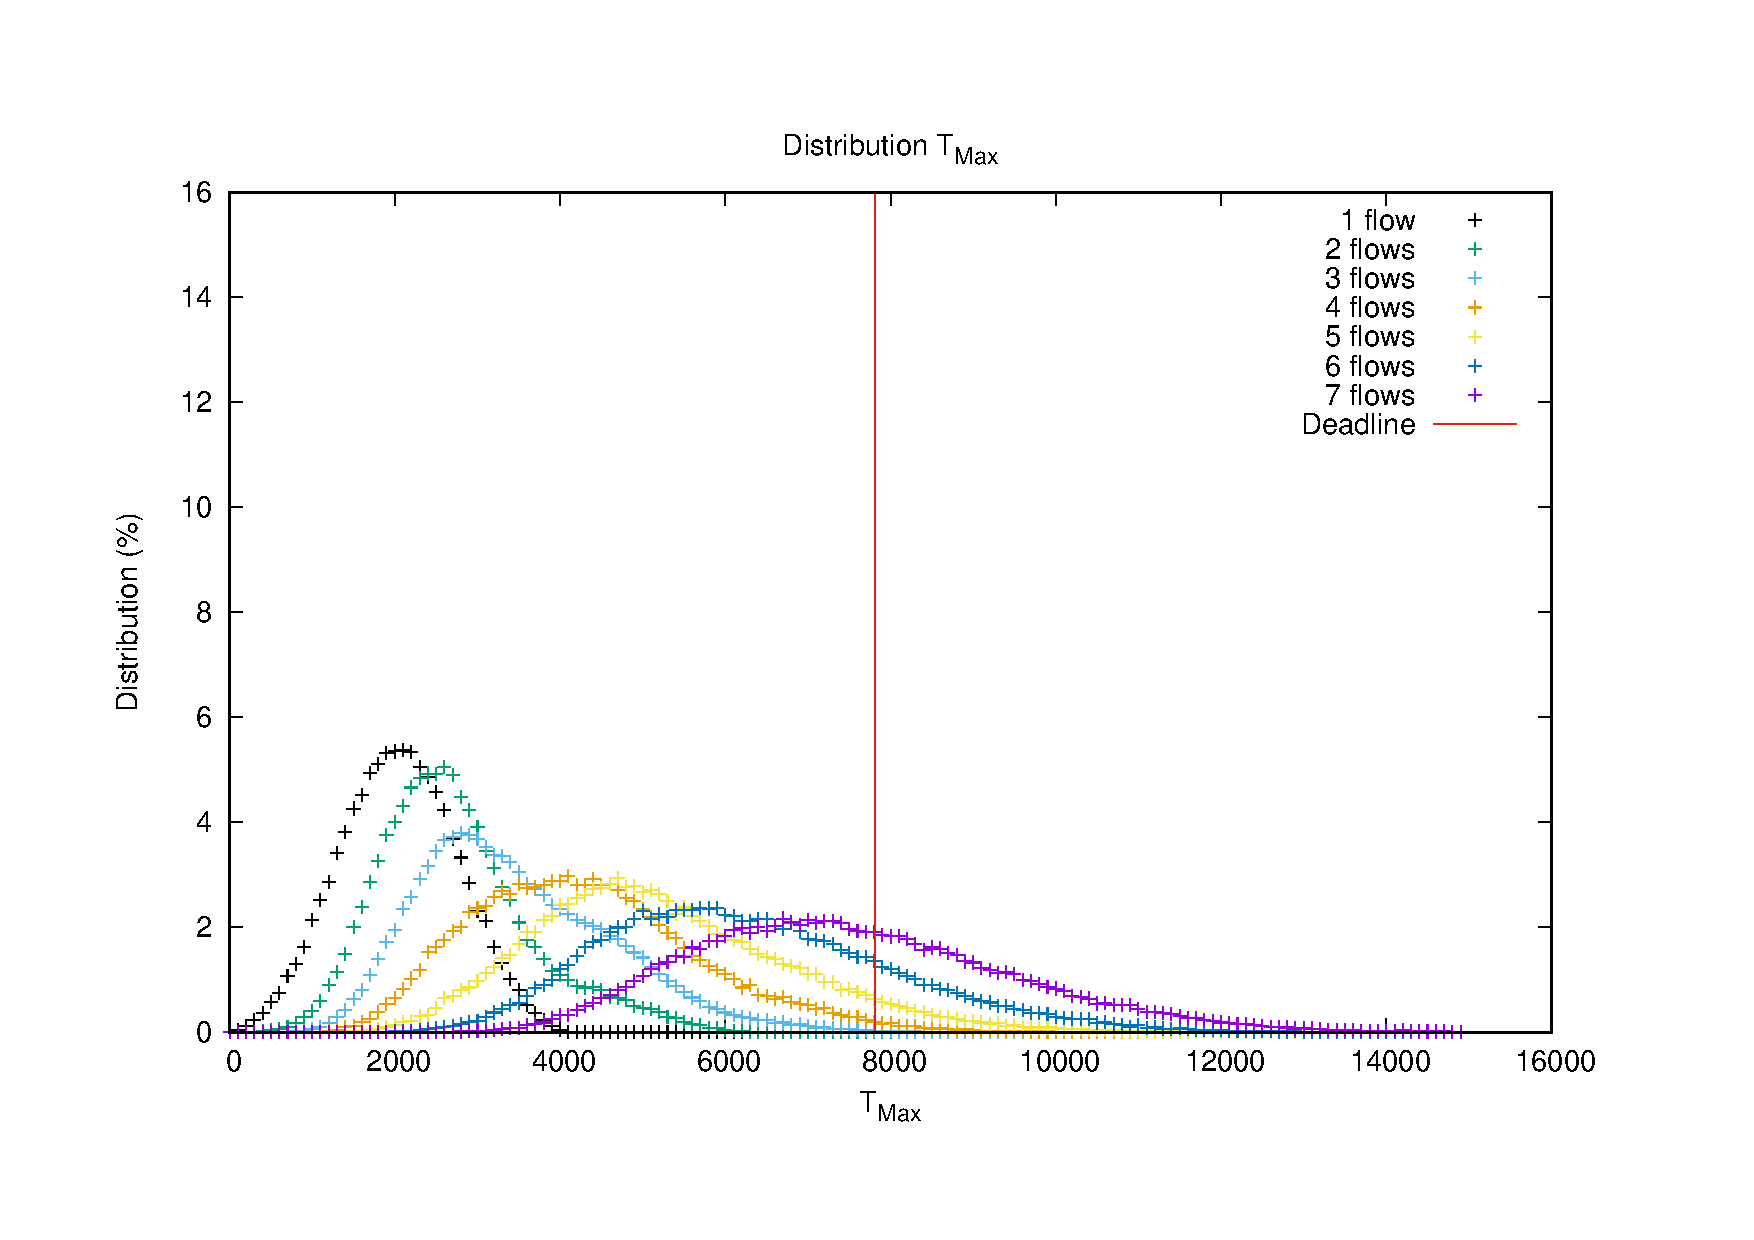
\includegraphics[scale=0.6]{distributions_random.pdf}%scale=0.6
\caption{Distributions for random sending}
\end{figure}

For LSG, the major part of the solutions are giving $T_{max} \simeq 2500-3000$, and there is no
solution with $T_{max}$ exceeding $\simeq 4000$ slots.
The random sending is giving more distributed results. A lot of cases gives us some $T_{max} >$ deadline for 3 flows or more.
The cumulative distribution (cf Appendix Fig 5 and 6) shows us that with 7 flows, we have $\simeq 60\%$ of the cases in which $T_{max} >$ deadline


\end{subsection}

\end{section}

\begin{section}{Synthesis}
Finding a solution without waiting time would be the perfect solution to solve our problem because it guarantees us the minimal latency.

To find such a solution, we proposed four algorithms. The first one has theoretical certitudes but practical bad results (Greedy Star).
For the Shortest Longest Algorithm we can calculate the period depending of the difference between the longest and the shortest route.
In our situation, this algorithm gives us good results because that difference is not too large.
Then, the Greedy Prime algorithm finds some good solutions close to the lower bound but still worse than the Exhaustive Generation.
We observed that for those parameters, Shortest Longest is giving optimal solutions, like the Exhaustive Generation.

Furthermore, finding a solution without waiting times involve to get a large enough period. Considering our problem, we noticed that when the 
load increases, there are some cases in which a solution without waiting time does not exists.

Thus, by allowing the messages to be buffered in source nodes with LSG, we find good solutions satisfying our latency 
criteria in the given period. To prove that this algorithm is useful, we compared the results of LSG with the results of some
random messages sending managed with some buffers in switches. The results have proven that LSG is useful, if we want
to satisfy the latency constraint.

\end{section}

\end{chapter}



\begin{chapter}{Conclusion}

This study took place in a collaboration between Nokia Bell Labs France and the DAVID laboratory.
A previous work about the study of the complexity of the general case (topology 3) was made before this work.
In the first month, the main objective was to define the problem with the specifications corresponding to the reality.
In parallel, we started to study some related works and to try finding some ideas and approaches. That is the reason why some articles are not related
with the first topology on which we worked in that study, but on the current case.

The precise definition of this problem opened a lot of questions on the first topology, that is why we only studied it.

Then we proposed a first approach to solve this scheduling problem, without considering waiting times. We saw with the simulations 
that this approach gives us satisfying results until the load of the network is not too high.
The second approach, which is to allow waiting time and to find a good heuristic to schedule the messages respecting the latency constraint,
gave us good solution, compared to our experimental random sending, that correspond to the nowadays way to manage the network.

In this report, we studied the topology 1 with some given parameters, corresponding to the reality. Some of these parameters, in particular the fact that the travel time of the routes are shorter than the time to emit a message involves some particular cases results. We can imagine that the results of the Shortest Longest, for example, could be notably different with longer routes.
We can improve our model with some variant to allow the problem to be closer to the reality. In real networks, all the links does not have the same bandwidth. Also, the computation time $\theta$ could change according to the routes, and not be simplified.

As well, we can imagine using some of these results and algorithm on the others topologies, by finding some common property between the optical ring topology and the topology 1 that we studied.
\end{chapter}
\appendix

\chapter*{Appendix}
\addcontentsline{toc}{chapter}{Appendix}

 
\begin{figure}[H]
\hspace*{-3cm}
\centering
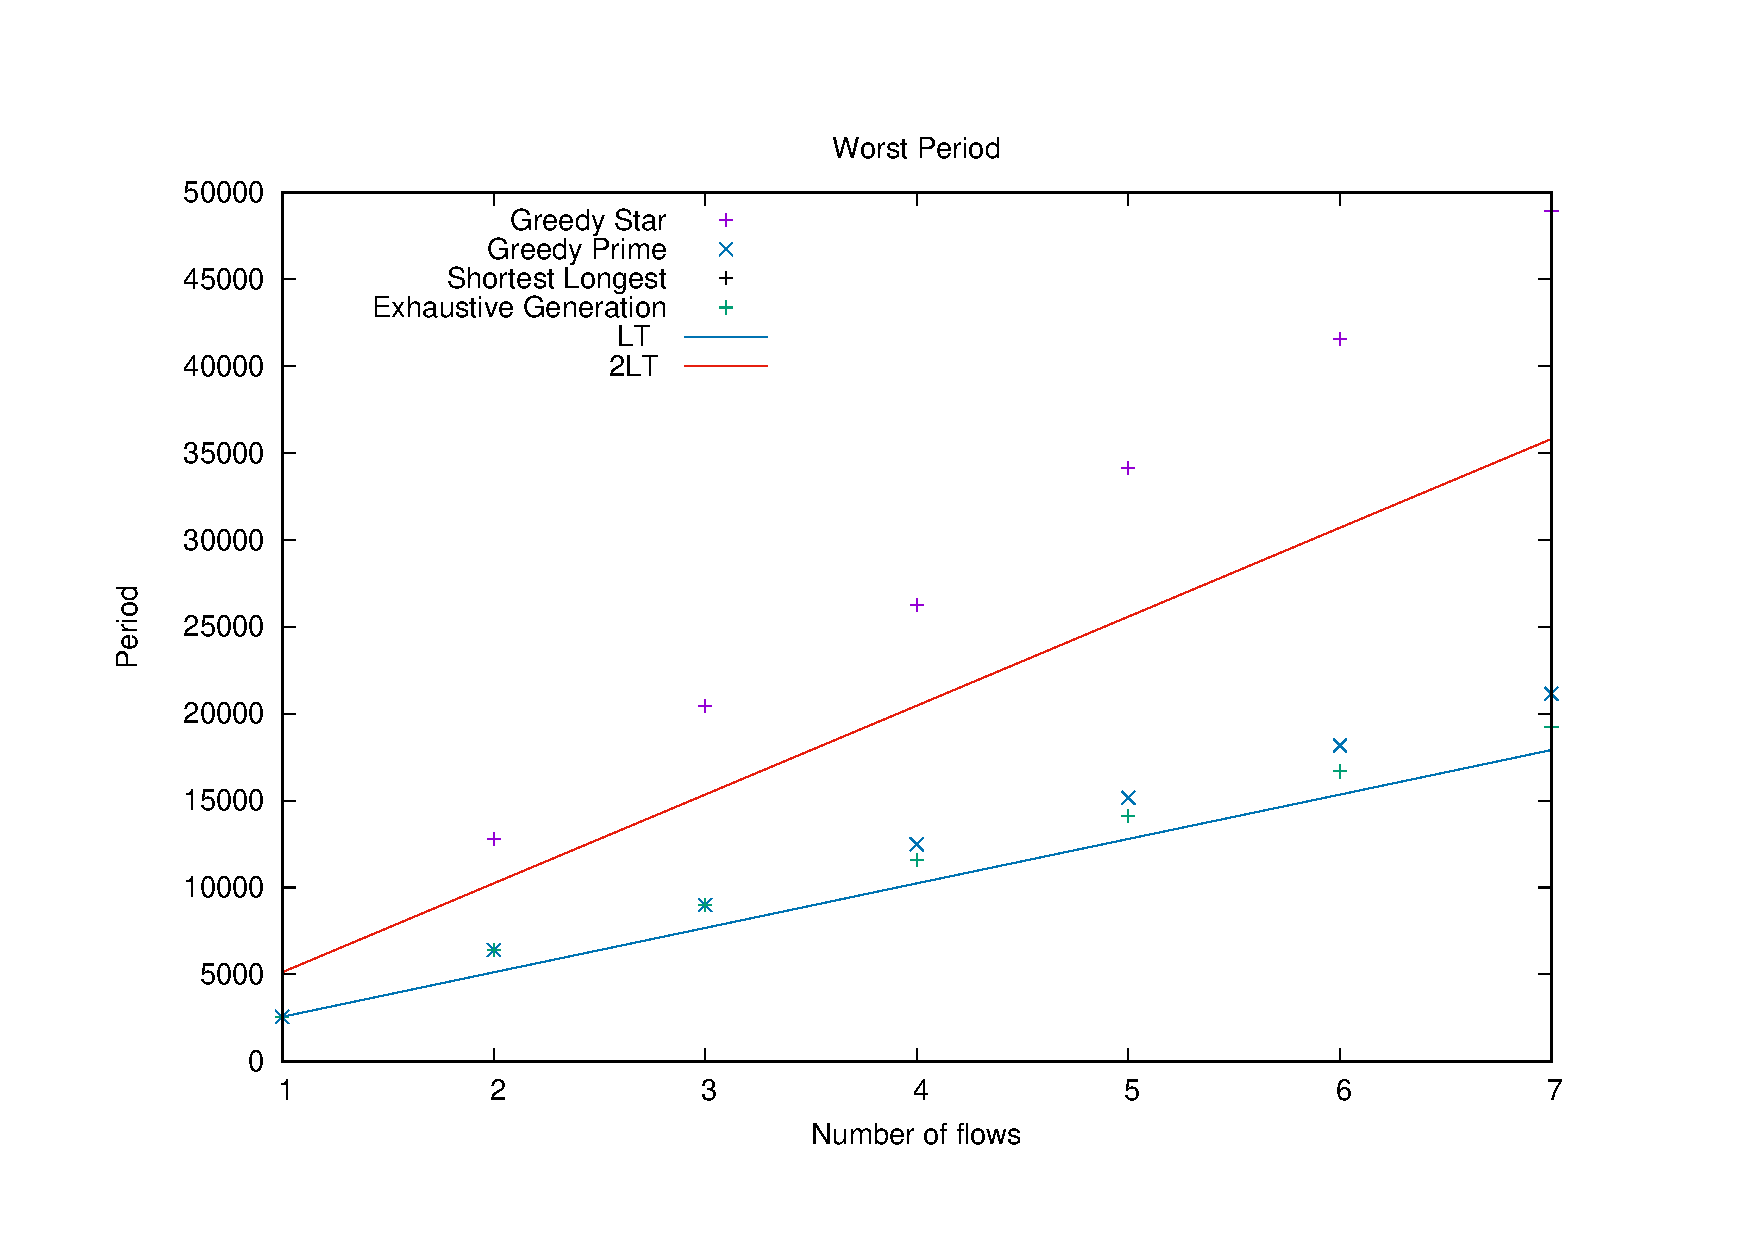
\includegraphics[scale=0.6]{windowworst.pdf}%scale=0.6
\caption{Worst periods for algorithms without waiting times}
\end{figure}

\begin{figure}[H]
\hspace*{-3cm}
\centering
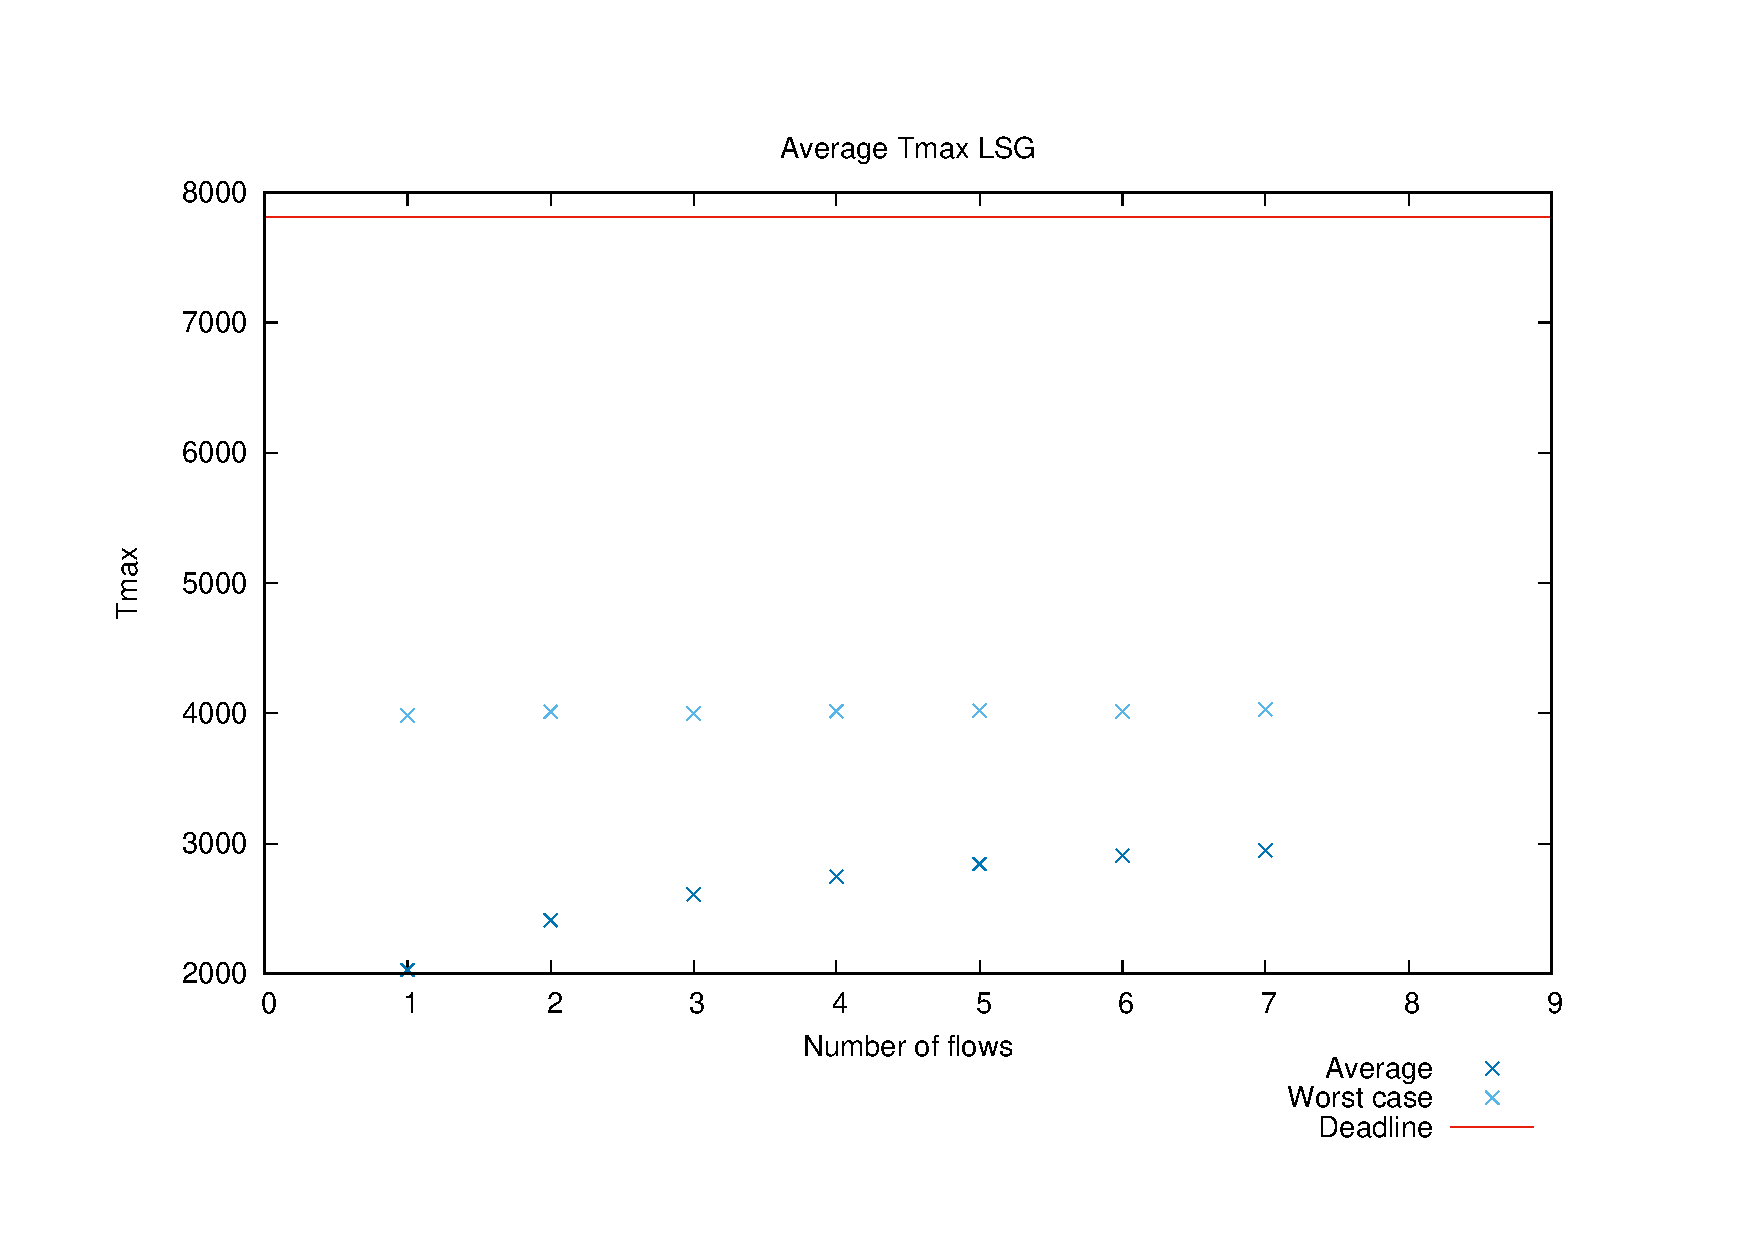
\includegraphics[scale=0.6]{tmaxlongest.pdf}%scale=0.6
\caption{$T_{max}$ with LSG}
\end{figure}

\begin{figure}[H]
\hspace*{-3cm}
\centering
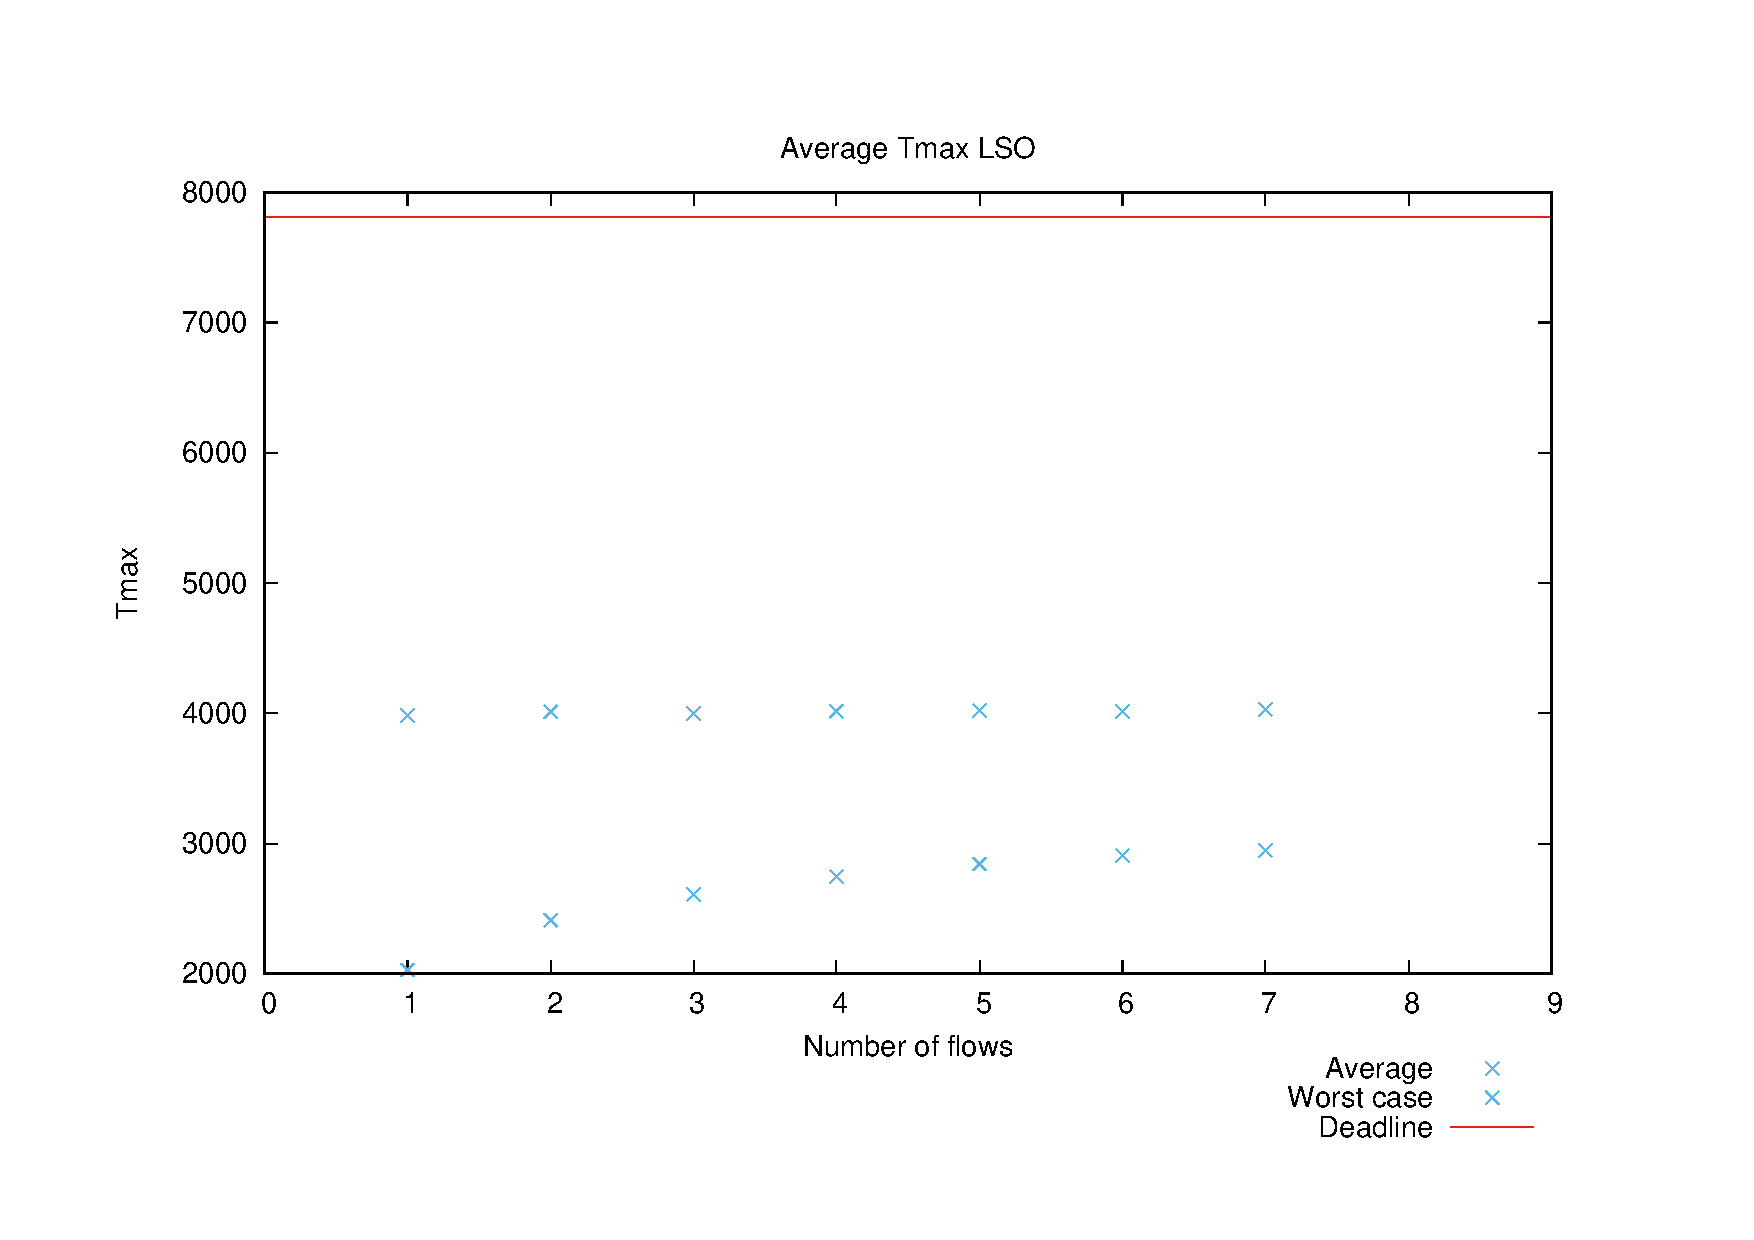
\includegraphics[scale=0.6]{tmaxsimons.pdf}%scale=0.6
\caption{$T_{max}$ with LSO}
\end{figure}


\begin{figure}[H]
\hspace*{-3cm}
\centering
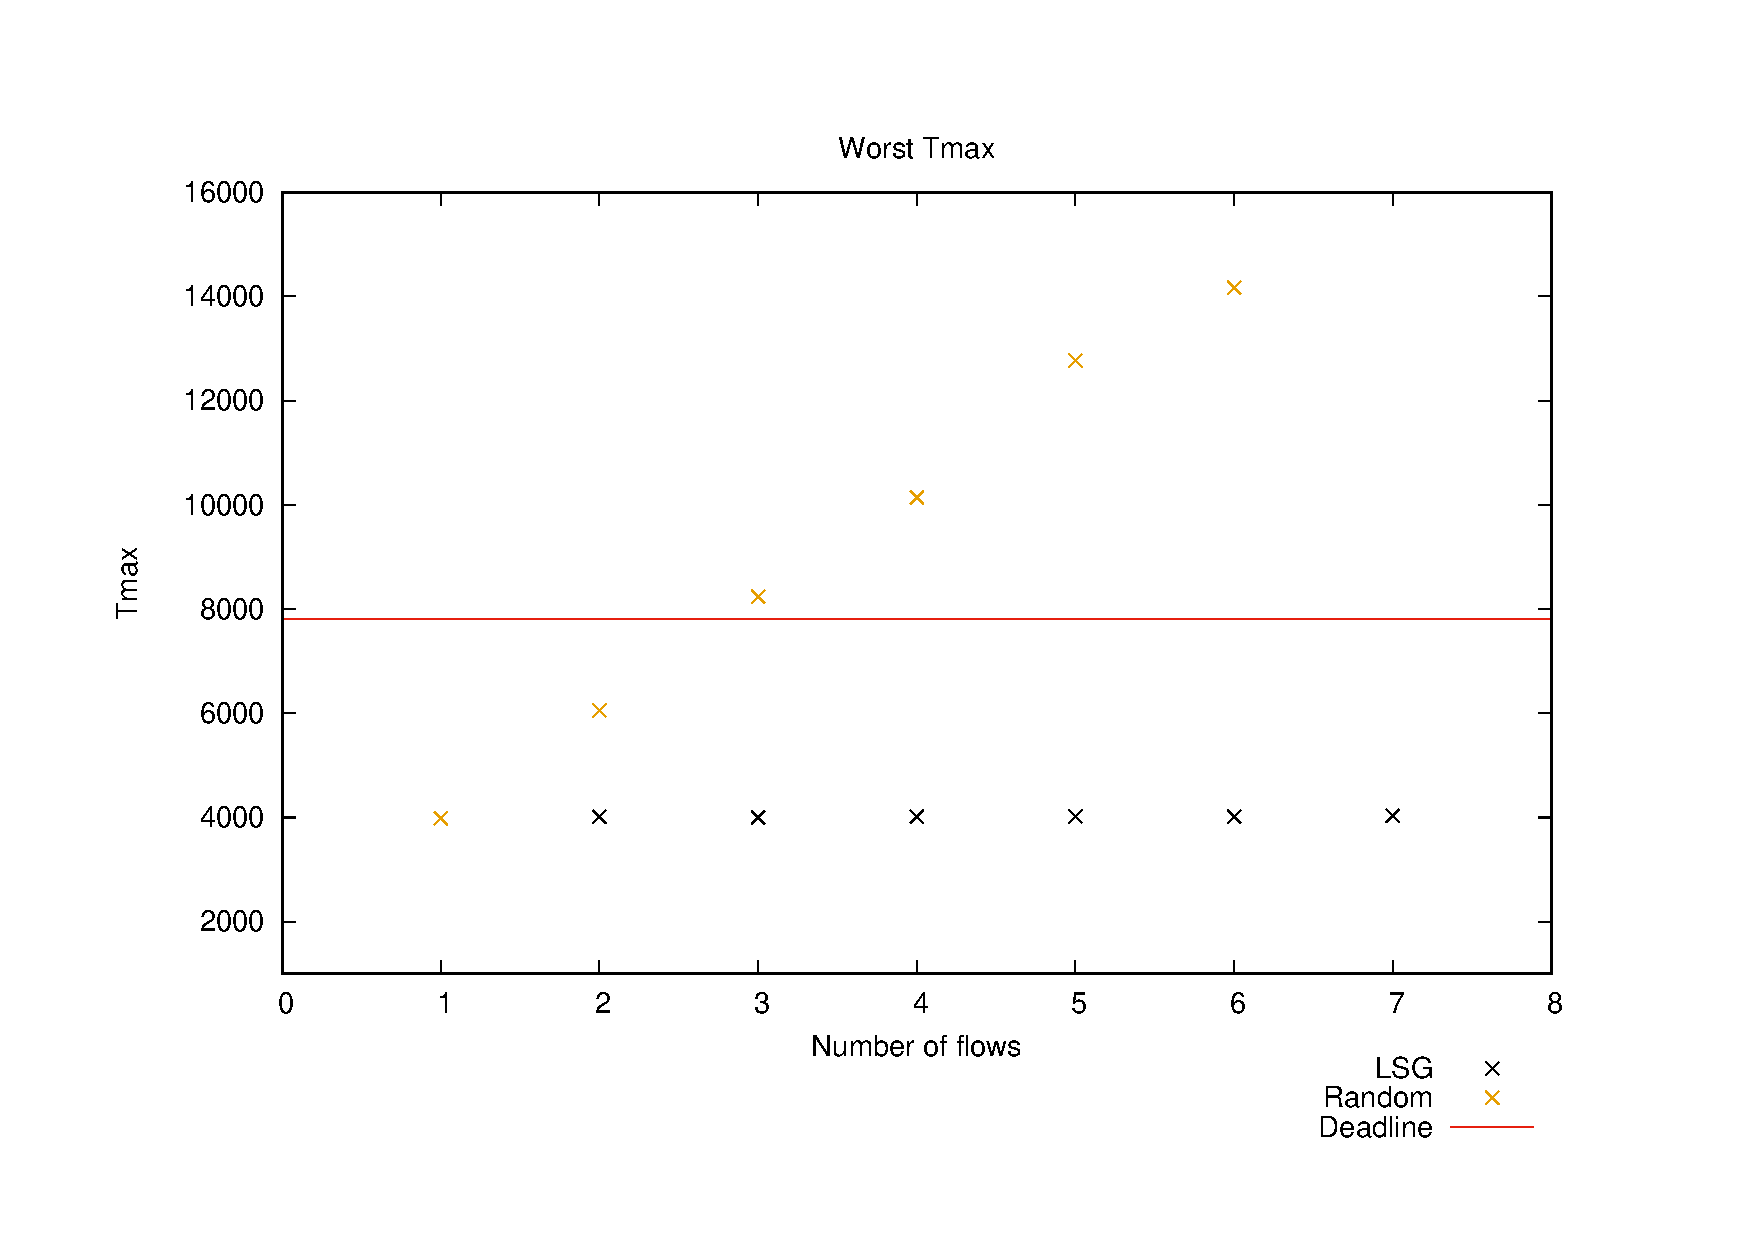
\includegraphics[scale=0.6]{tmax0worst.pdf}%scale=0.6
\caption{Worst $T_{max}$ with Random and LSG}
\end{figure}


\begin{figure}[H]
\hspace*{-3cm}
\centering
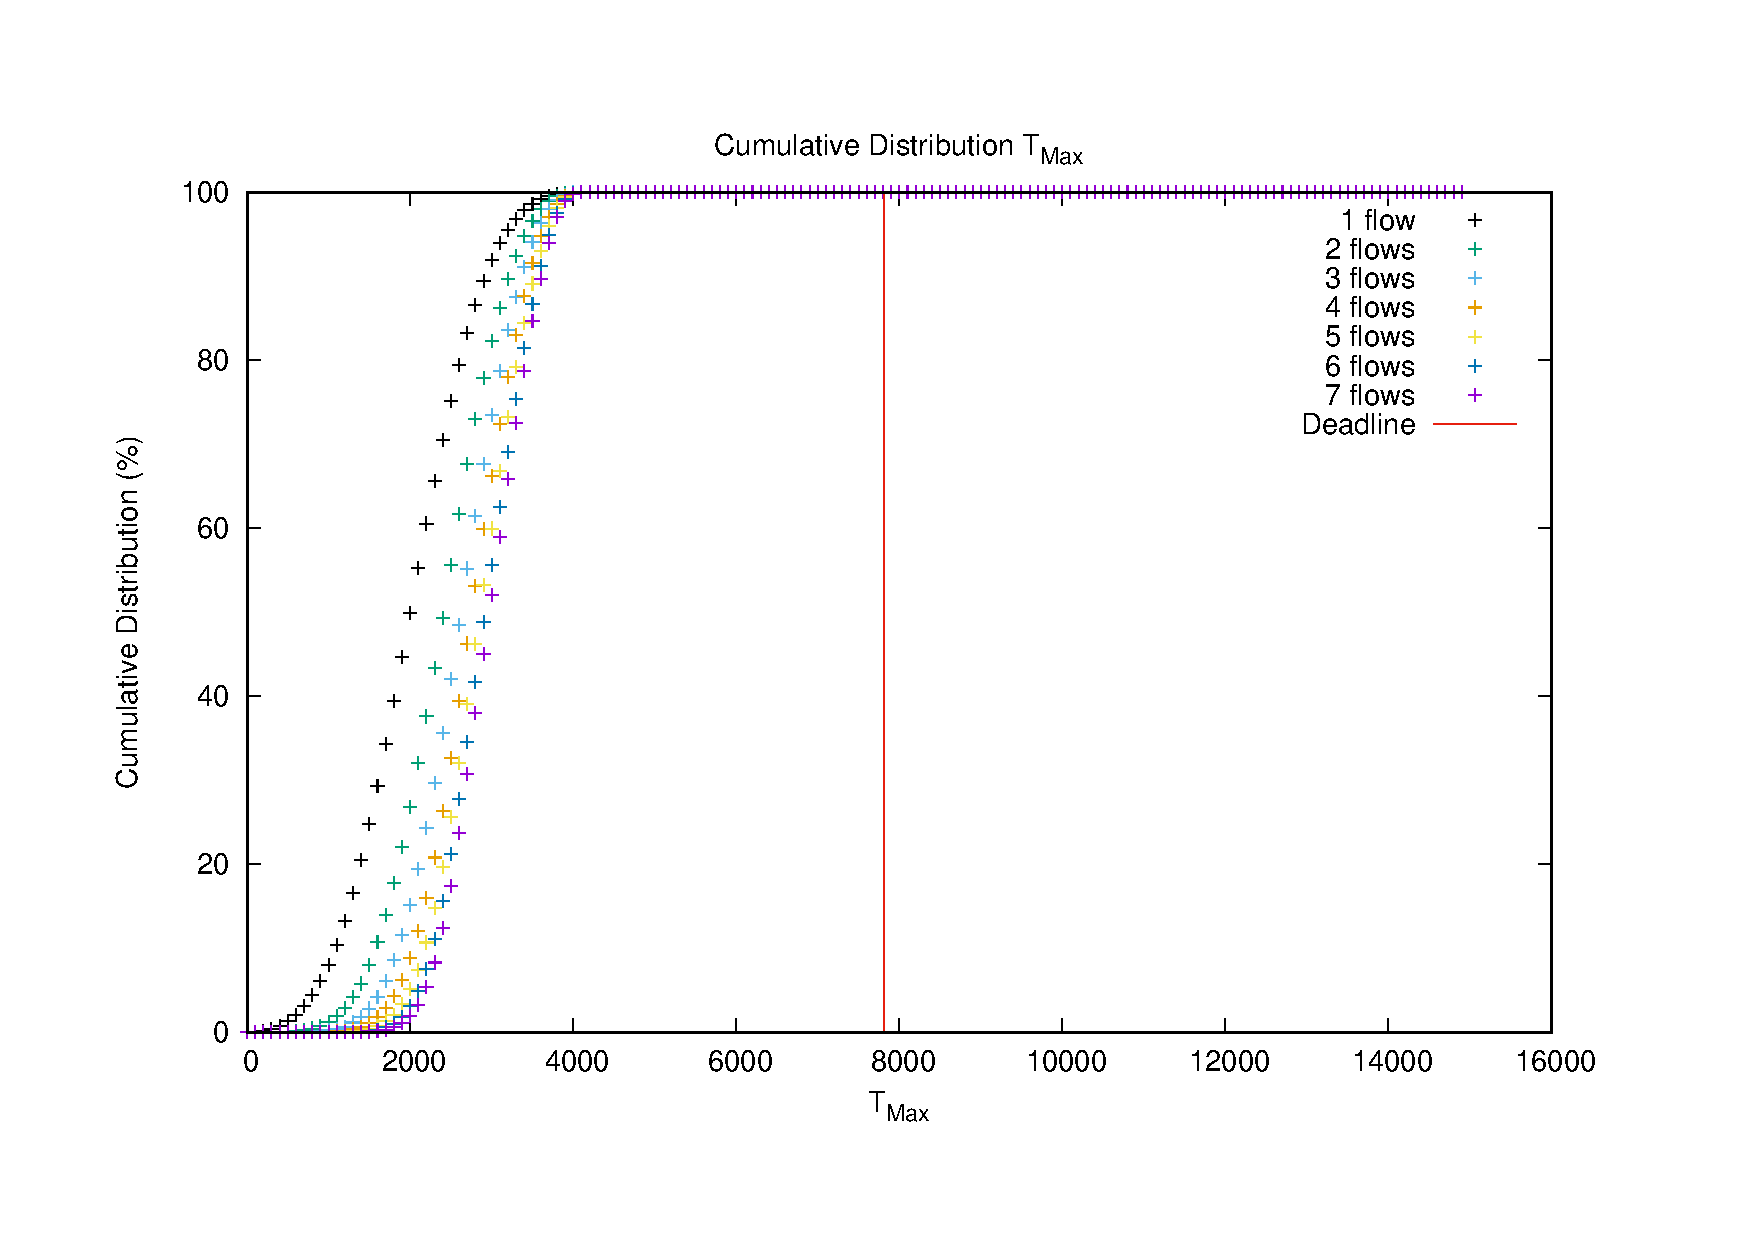
\includegraphics[scale=0.6]{distriscumul_longest.pdf}%scale=0.6
\caption{Cumulative distributions For LSG}
\end{figure}

\begin{figure}[H]
\hspace*{-3cm}
\centering
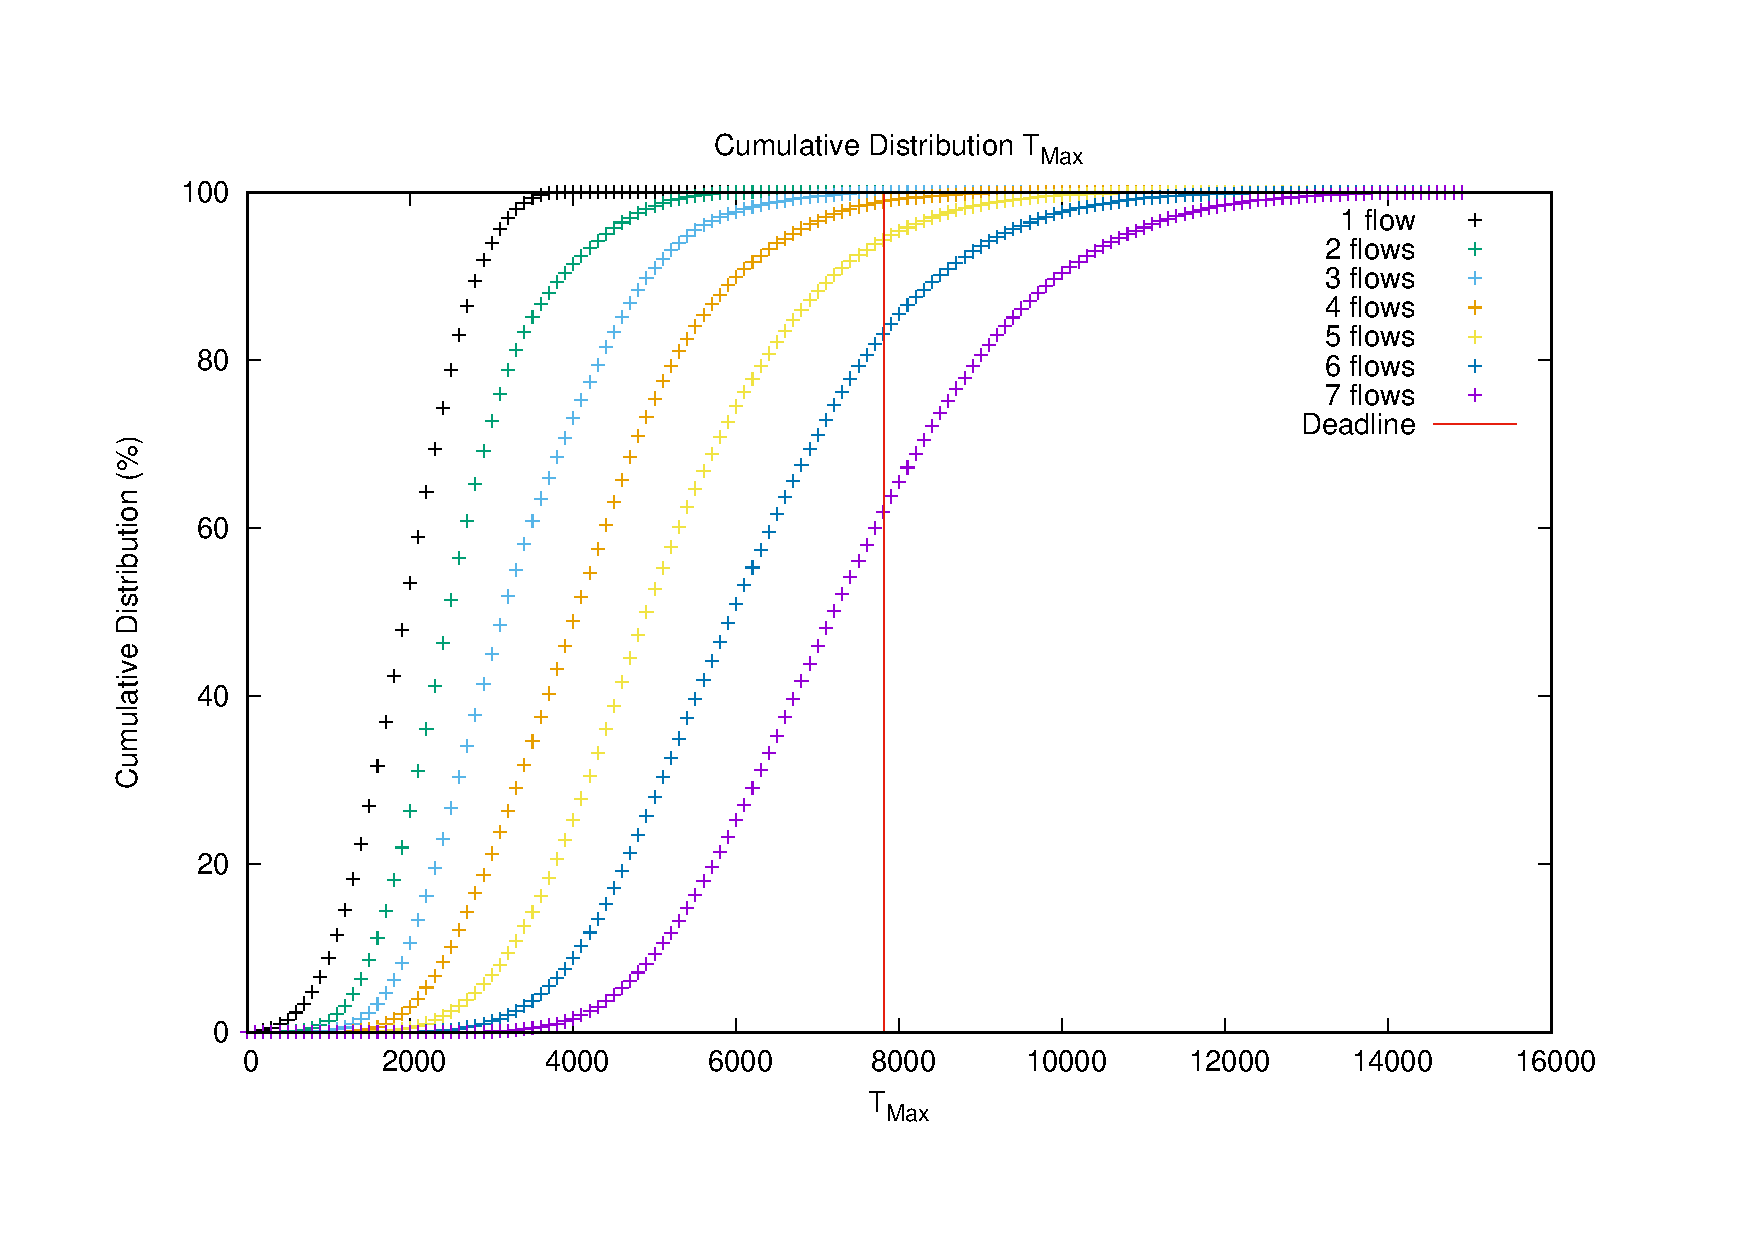
\includegraphics[scale=0.6]{distriscumul_random.pdf}%scale=0.6
\caption{Cumulative distributions For Random}
\end{figure}


\bibliographystyle{plain}
\bibliography{Sources}
\addcontentsline{toc}{chapter}{Bibliography}
\end{document}
